%% =========================================================================
%%  JUCO — Complete Manuscript
%%  Journal  : Artificial Intelligence in Medicine (Elsevier)
%%  Template : Elsevier CAS (cas-sc.cls — single-column)
%%  Compiled : pdflatex → bibtex → pdflatex × 2
%%
%%  Download template :
%%  https://assets.ctfassets.net/o78em1y1w4i4/5uFmLZJTPDMAUjFnHRpjj8/
%%  6f19a979146eb93263763d87a894ab0d/els-cas-templates.zip
%% =========================================================================

\documentclass[a4paper,fleqn,longmktitle]{cas-sc}

%% ── Required packages ────────────────────────────────────────────────────
%% NOTE: cas-sc.cls already loads: graphicx, amsmath/amssymb/amsfonts,
%%       booktabs, multirow, xcolor (svgnames), hyperref (colorlinks).
%%       Only load packages NOT provided by the class.
\usepackage{url}               % \url{}
\usepackage{natbib}            % author-year citations
\usepackage[expansion=false]{microtype}  % protrusion only
\usepackage{enumitem}          % list control
%\usepackage{amsthm}  % CAS 2024 provides theorem machinery
\usepackage{algorithm}         % algorithm float
\usepackage{algpseudocode}     % pseudocode
\usepackage{placeins}
%% Customise hyperref colors (cls already loaded hyperref with [colorlinks])
\usepackage{nonfloat}

\AtBeginDocument{%
	\hypersetup{hypertexnames=false,
		linkcolor=blue!60!black,
		citecolor=green!50!black,
		urlcolor=blue!70!black}%
}

%% ── Theorem environments ─────────────────────────────────────────────────
\newtheorem{problem}{Problem}

\setlength{\textfloatsep}{16pt}
\setlength{\floatsep}{6pt}
\setlength{\intextsep}{6pt}
\setlength{\belowcaptionskip}{0pt}
\setlength{\abovecaptionskip}{0pt}
%% =========================================================================
\begin{document}
	%% =========================================================================
	
	
	%% ── Title ─────────────────────────────────────────────────────────────────
\title{JUCO: A Joint Uncertainty-Calibrated Optimisation Framework with
	Fuzzy Decision Forests and Safe Abstention for ICU Mortality
	Prediction Under Informative Missingness}
\shorttitle{JUCO: Fuzzy Decision Forests for ICU Mortality Under Informative Missingness}
	
	%% Running head author line (use lead author et al.)
	\shortauthors{Avoy et al.}
	
	%% ── Authors ───────────────────────────────────────────────────────────────
	%% Three authors: two co-authors (students/researchers) + one faculty supervisor
	%% Replace all [PLACEHOLDER] fields before submission
	

\author[1]{Avoy Nath Chowdhury}[orcid=0009-0001-2345-6789]
\cormark[1]
\ead{avoynath2004@gmail.com}

\author[1]{Anik Sarker}[orcid=0000-0000-0000-0000]
\ead{23053402@kiit.ac.in}

\author[1]{Niloy Deb}[orcid=0000-0000-0000-0000]
\ead{23053552@kiit.ac.in}

\author[2]{Anisha Kumari}[orcid=0000-0000-0000-0000]
\ead{anishamishracs@gmail.com}
\cortext[1]{Corresponding author. \href{mailto:avoynath2004@gmail.com}{avoynath2004@gmail.com}}

\address[1]{School of Computer Engineering, KIIT Deemed to be University,
	Bhubaneswar, Odisha, India}
\address[2]{Department of Computer Science and Engineering, Motilal Nehru National Institute of Technology, Allahabad, Uttar Pradesh India}
	

	%% ── Abstract (≤ 250 words — AIM hard limit) ───────────────────────────────
	\begin{abstract}
		\leavevmode\textbf{Background.}
		ICU mortality prediction models trained on electronic health records
		face pervasive Missing-Not-At-Random (MNAR) data caused by
		selective clinical test ordering.
		Standard gradient boosting methods achieve competitive discrimination
		within their training distribution by treating missingness as a
		proxy variable, but degrade substantially when missingness patterns
		shift between institutions.
		No existing framework simultaneously quantifies imputation
		uncertainty, propagates it structurally to a downstream classifier,
		and converts it into principled prediction abstention.
		
		\textbf{Methods.}
		We introduce JUCO (Joint Uncertainty-Calibrated Optimisation),
		a four-phase framework.
		LightGBM quantile regression produces interval-valued imputations
		$[q^L, q^U]$ rather than point estimates.
		Intervals are encoded as trapezoidal fuzzy numbers whose support
		width represents imputation uncertainty.
		A fuzzy decision forest soft-routes samples, down-weighting imputed
		inputs in leaf votes.
		An entropy-based safe abstention protocol defers high-uncertainty
		predictions to clinician review.
		All five hyperparameters are jointly optimised via two-stage
		Differential Evolution on MIMIC-IV, then frozen for external
		validation on eICU (208 hospitals).
		
		\textbf{Results.}
		Under escalating MNAR stress (10\%--70\%), JUCO's AUROC degrades
		by $-0.023$ versus $-0.054$ for XGBoost and $-0.056$ for
		MissForest+XGB; JUCO overtakes both at 70\% missingness
		($0.799$ vs $0.795$ and $0.792$).
		Safe abstention yields a $2.8{\times}$ AURC reduction versus
		full-coverage prediction ($0.032$ vs $0.090$).
		Under standard 30\% MNAR, the AUROC gap between gradient boosting
		and JUCO narrows by 46\% from MIMIC-IV to eICU ($-0.028$ to
		$-0.015$), consistent with missingness exploitation diminishing
		under cross-institutional shift.
		
		\textbf{Conclusions.}
		JUCO provides principled uncertainty propagation from missing data
		to clinical prediction deferral, offering the greatest advantage
		in environments where data pipeline integrity cannot be guaranteed.
		Code available at \url{https://github.com/[REDACTED-BEFORE-SUBMISSION]}.
	\end{abstract}
	
	%% ── Keywords ──────────────────────────────────────────────────────────────
	\begin{keywords}
		ICU mortality prediction \sep
		missing not at random \sep
		fuzzy decision forest \sep
		uncertainty quantification \sep
		selective prediction \sep
		electronic health records
	\end{keywords}
\maketitle
	
	
	%% ── Highlights (AIM strongly encourages; ≤ 5 bullets, ≤ 85 chars each) ──
	%% Place in a SEPARATE editable file named "Highlights.docx" at submission
	%% Content (copy to that file):
	%%
	%%   • JUCO propagates imputation uncertainty through fuzzy trees to abstention
	%%   • AUROC degrades –0.023 vs –0.054 for XGBoost under 70% MNAR stress
	%%   • Safe abstention cuts AURC by 2.8x vs full-coverage prediction
	%%   • AUROC gap narrows 46% on eICU: missingness exploitation is brittle
	%%   • Joint differential evolution optimises all four phases end-to-end
	%%
	%% ────────────────────────────────────────────────────────────────────────────
	
	
	%% =========================================================================
	%%  SECTION 1 — INTRODUCTION
	%% =========================================================================
	
	\section{Introduction}
	\label{sec:introduction}
	
	Accurate prediction of in-hospital mortality for ICU patients
	enables early intervention, targeted resource allocation, and timely
	initiation of goals-of-care conversations.
	Over the past decade, machine learning models trained on electronic
	health records (EHR) — particularly gradient boosting methods —
	have achieved discrimination levels comparable to established clinical
	scores such as APACHE and
	SOFA~\citep{purushotham2018benchmarking, johnson2023mimic},
	with AUROC values routinely in the range 0.82--0.88 on
	retrospective cohorts.
	Yet deployment of these models in real ICU environments
	remains limited~\citep{topol2019high}, and a persistent
	obstacle is the pervasive, structured missingness of EHR data.A recent meta-analysis of 40 ICU mortality prediction studies
	confirms gradient boosting as the dominant modality, yet
	identifies systematic calibration deficits as the primary
	unresolved limitation~\citep{sun2025meta}.
	
	ICU laboratory and vital sign measurements are not missing at random.
	A clinician's decision to order a lactate measurement, a blood
	culture, or an arterial blood gas is itself a clinical judgment
	driven by patient acuity — the probability that a value is
	measured is correlated with the value itself and with the
	patient's probability of death.
	This Missing-Not-At-Random (MNAR) mechanism~\citep{rubin1976inference}
	means that the \emph{absence} of a measurement carries prognostic
	information, and that the distribution of missing data at test time
	may differ from training time as hospital protocols, equipment,
	staffing, and patient populations evolve.
	Benchmark studies confirm that clinical risk models degrade
	systematically when evaluated on external
	populations~\citep{moons2012risk}, and recent work attributes
	a significant fraction of this degradation to unstable missingness
	patterns~\citep{agniel2018biases, josse2019consistency}.
	
	Existing approaches to missing data in clinical ML occupy two extremes
	that both fail to address this challenge fully.
	\emph{Point imputation methods} — mean imputation, MICE,
	MissForest — produce single values for each missing entry and discard
	uncertainty, giving downstream classifiers no mechanism to distinguish
	confidently observed features from highly uncertain imputed ones.
	\emph{Native NaN routing} in gradient boosting methods
	(XGBoost~\citep{chen2016xgboost},
	LightGBM~\citep{ke2017lightgbm}) avoids imputation entirely
	but encodes the MNAR structure as a proxy variable whose stability
	depends on the stationarity of the missingness mechanism between
	training and deployment.
	Neither approach quantifies imputation uncertainty, neither propagates
	it structurally to the classifier, and neither provides a mechanism
	for identifying and deferring predictions when imputation quality
	is low.
	In safety-critical deployment, this is a failure mode: a model that
	issues a confident mortality prediction for a patient whose key
	laboratory values are all imputed provides false certainty that can
	harm rather than help clinical decision-making.
	
	We introduce \textbf{JUCO} (\textbf{J}oint
	\textbf{U}ncertainty-\textbf{C}alibrated \textbf{O}ptimisation),
	a four-phase framework that treats imputation uncertainty as a
	first-class quantity throughout the prediction pipeline.
	The key insight is that a quantile regression interval
	$[q^L, q^U]$ directly encodes imputation confidence: a wide
	interval indicates low confidence, a narrow interval high confidence.
	Encoding this interval as a trapezoidal fuzzy number and routing
	samples \emph{softly} through a decision tree — so uncertain
	samples split their weight across both children in proportion to
	their uncertainty — propagates imputation quality to the tree's
	leaf distribution.
	The resulting entropy of the leaf distribution then drives abstention:
	high entropy triggers deferral to clinical review.
	This chain — from missing data to interval to fuzzy number to soft
	routing to entropy to abstention — is end-to-end, structurally
	motivated, and jointly optimised via Differential Evolution.
	
	We evaluate JUCO on MIMIC-IV~\citep{johnson2023mimic}
	(82{,}785 ICU stays, Beth Israel Deaconess Medical Center)
	as a primary cohort and on the eICU Collaborative Research
	Database~\citep{pollard2018eicu}
	(162{,}136 stays across 208 US hospitals) as an external
	validation cohort with parameters frozen from MIMIC-IV training.
	Under escalating informative missingness (10\%--70\%), JUCO's
	AUROC degrades by $-0.023$, compared to $-0.054$ for XGBoost
	and $-0.056$ for MissForest+XGB; JUCO overtakes both models at
	70\% missingness ($0.799$ vs $0.795$ and $0.792$).
	The safe abstention protocol reduces AURC by $2.8{\times}$ versus
	full-coverage prediction ($0.032$ vs $0.090$).
	Under standard 30\% MNAR, gradient boosting achieves statistically
	significantly higher AUROC than JUCO ($0.842$ vs $0.814$,
	DeLong $z = -18.04$, $p < 0.001$); this gap narrows by 46\% on
	eICU ($-0.028$ MIMIC-IV vs $-0.015$ eICU), consistent with
	gradient boosting's missingness-exploitation advantage diminishing
	under cross-institutional distributional shift.
	
	The specific contributions of this paper are:
	\begin{enumerate}
		\item A four-phase framework that structurally propagates
		quantile-regression imputation uncertainty through a fuzzy
		decision forest to entropy-based clinical abstention,
		jointly optimised end-to-end via two-stage Differential
		Evolution.
		
		\item A systematic missingness stress test across seven MNAR rates
		(10\%--70\%) demonstrating that JUCO's graceful degradation
		($\Delta\text{AUROC} = {-}0.023$) is substantially smaller
		than gradient boosting baselines ($-0.054$ to $-0.056$).
		
		\item An ablation study isolating each architectural component:
		the safe abstention protocol ($2.8{\times}$ AURC improvement) and
		fuzzy soft routing (12.7\% ECE reduction vs crisp routing).
		
		\item Transparent reporting of JUCO's lower nominal AUROC under
		standard conditions with a mechanistic explanation based on
		gradient boosting's use of missingness as a stationary
		proxy variable, and empirical evidence that this advantage
		diminishes under distributional shift.
		
		\item Cross-institutional external validation on eICU with frozen
		parameters demonstrating a 46\% reduction in the AUROC gap.
	\end{enumerate}
	
	The remainder of this paper is organised as follows.
	Section~\ref{sec:related_work} surveys related work.
	Section~\ref{sec:problem_formulation} formalises the problem.
	Section~\ref{sec:methodology} describes the JUCO architecture.
	Section~\ref{sec:experimental_setup} describes datasets, protocol,
	and baselines.
	Section~\ref{sec:results} presents experimental results.
	Section~\ref{sec:discussion} discusses findings and limitations.
	Section~\ref{sec:conclusion} concludes.
	This study follows the \textsc{tripod+ai} reporting
	guidelines for clinical prediction models~\citep{collins2024tripodai}.
	
	%% =========================================================================
	%%  SECTION 2 — RELATED WORK
	%% =========================================================================
	
	\section{Related Work}
	\label{sec:related_work}
	
	This section surveys four bodies of literature that directly
	motivate and situate the contributions of this paper:
	missing data in EHR-based clinical prediction, imputation
	under informative missingness, fuzzy set methods for
	uncertain data, and selective prediction with abstention.
	
	\subsection{Missing Data in ICU Clinical Prediction}
	\label{sec:rw_missing}
	
	Electronic health records contain pervasive missingness by design:
	clinicians order tests selectively based on patient acuity,
	meaning the decision to measure a variable is correlated with
	the variable's value and the patient's
	outcome~\citep{agniel2018biases}.
	This produces a Missing-Not-At-Random (MNAR) mechanism in the
	formal sense of \citet{rubin1976inference}: the probability
	that an entry is missing depends on the missing value itself,
	not only on observed data.
	Standard missing-at-random (MAR) or missing-completely-at-random
	(MCAR) assumptions that underpin most imputation methods are
	therefore violated in ICU data, with consequences for both
	imputation quality and downstream model validity.
	
	Benchmark studies on MIMIC-III/IV have demonstrated that gradient
	boosting methods — particularly XGBoost and LightGBM — achieve
	competitive ICU mortality prediction performance~\citep{johnson2016mimic,johnson2023mimic,
		purushotham2018benchmarking}, with AUROC values in the range 0.82--0.88.
	These methods handle missingness implicitly through learned
	NaN routing: split directions for missing entries are determined
	during training to minimise loss, effectively treating the absence of a measurement as a
	learnable feature~\citep{chen2016xgboost}.
	While this approach is efficient and often effective within a
	single institution's stable data pipeline~\citep{perezlebel2022benchmarking},
	it encodes the missingness structure as a proxy variable
	whose validity depends on the stationarity of the MNAR
	mechanism~\citep{josse2019consistency,perezlebel2022benchmarking}.
	When the deployment environment differs from training —
	different hospital charting protocols, data pipeline failures,
	or equipment changes — the learned NaN routing becomes
	miscalibrated~\citep{sperrin2020informative}.
	Our stress test results (XGBoost $\Delta\text{AUROC} = -0.054$
	at 70\% MNAR vs JUCO $-0.023$) are consistent with this fragility.
	
	\subsection{Imputation Methods for Informative Missingness}
	\label{sec:rw_imputation}
	
	Standard imputation approaches for clinical data include mean/median
	imputation~\citep{sterne2009multiple}, multiple imputation by chained
	equations (MICE~\citep{van2011mice}), and
	MissForest~\citep{stekhoven2012missforest}.
	All of these produce point estimates and discard uncertainty
	information, leaving the downstream classifier unable to distinguish
	between confidently imputed and highly uncertain entries.
	
	Deep generative approaches address this limitation by modelling
	the full conditional distribution of missing values.
	\citet{yoon2018gain} propose GAIN, a GAN-based imputation method.
	\citet{ipsen2020not} extend variational autoencoders to MNAR data,
	producing distributional imputations.
	\citet{ma2020mimic} use recurrent networks with explicit missingness
	modelling for temporal EHR data.
	More recently, \citet{zhao2024multitask} propose a multi-task
	diffusion model for mortality prediction with incomplete data in
	shock patients.
	These approaches produce richer uncertainty representations, but
	they do not propagate imputation uncertainty to the classification
	stage and do not incorporate abstention.
	
	Quantile regression provides an efficient alternative for
	interval-valued imputation~\citep{meinshausen2006quantile}.
	The key advantage is that prediction interval width directly
	encodes imputation uncertainty without distributional assumptions.
	To our knowledge, the present work is the first to use LightGBM
	quantile regression as an imputation engine whose output intervals
	are propagated through a downstream soft-routing classifier via a
	fuzzy transformation.
	
	\subsection{Fuzzy Set Methods for Uncertain Clinical Data}
	\label{sec:rw_fuzzy}
	
	Fuzzy set theory~\citep{zadeh1965fuzzy} provides a principled
	framework for reasoning about imprecise information.
	Trapezoidal fuzzy numbers have been applied to clinical decision
	support for representing measurement
	uncertainty~\citep{adlassnig1986fuzzy, torres2013fuzzy},
	but these applications use fuzzy representations at the rule level
	rather than as inputs to a learned classifier.
	Fuzzy decision trees with soft routing have been studied
	theoretically~\citep{olaru2003complete, yuan1995induction},
	but prior work has not addressed joint optimisation of imputation
	and tree hyperparameters, nor application to large-scale EHR data.
	\citet{hullermeier2021aleatoric} motivates the distinction between
	aleatoric and epistemic uncertainty that guides our design choices.
	
	\subsection{Selective Prediction and Safe Abstention}
	\label{sec:rw_selective}
	
	Selective prediction — the reject option — allows a model to
	withhold predictions for uncertain
	inputs~\citep{chow1957optimum, bartlett2008classification}.
	\citet{geifman2017selective} establish risk-coverage guarantees for
	selective prediction and introduce the AURC metric used in this paper.
	\citet{franc2023optimal} show that entropy is asymptotically optimal
	as an abstention criterion under a well-calibrated posterior.
	
	In clinical ML, \citet{jones2021selective} demonstrate entropy-based
	abstention for risk stratification, and \citet{kompa2021second}
	show AURC improvements across multiple clinical datasets.
	\citet{leibig2017leveraging} demonstrate that deferring uncertain
	predictions improves system-level accuracy in diabetic retinopathy
	screening.
	More recently, \citet{swaminathan2024selective} show that
	selective prediction reduces total misclassification cost in
	structured EHR data extraction tasks, demonstrating broad
	applicability of abstention in clinical ML pipelines.
	
	The key limitation of all prior clinical selective prediction work
	is that abstention is based on classification boundary uncertainty —
	not on uncertainty in the input features themselves.
	JUCO addresses this gap: wide imputation intervals produce wide fuzzy
	trapezoids, reduce split sharpness (Eq.~\ref{eq:sharpness}),
	produce diffuse leaf distributions, and increase output entropy.
	The abstention decision is mechanistically linked to imputation
	quality, not merely to the classification margin.
	
	
	%% =========================================================================
	%%  SECTION 3 — THEORY / PROBLEM FORMULATION
	%% =========================================================================
	
	\section{Problem Formulation}
	\label{sec:problem_formulation}
	
	\subsection{Clinical Setting and Notation}
	\label{sec:notation}
	
	Let $\mathcal{D} = \{(\mathbf{x}_i, \mathbf{M}_i, y_i)\}_{i=1}^{n}$
	denote a dataset of $n$ ICU stays, where:
	\begin{itemize}[noitemsep]
		\item $\mathbf{x}_i \in (\mathbb{R} \cup \{\text{NaN}\})^d$
		is the feature vector of $d$ clinical variables
		aggregated over the first 24 hours of admission;
		\item $\mathbf{M}_i \in \{0,1\}^d$ is the missingness indicator
		vector, with $M_{ij} = 1$ iff feature $j$ is missing;
		\item $y_i \in \{0, 1\}$ is the binary in-hospital mortality label.
	\end{itemize}
	
	Table~\ref{tab:notation} summarises all symbols used in this paper.
	
	\begin{table}[ht]
		\centering
		\caption{Summary of notation.}
		\label{tab:notation}
		\small
		\begin{tabular}{ll}
			\toprule
			\textbf{Symbol} & \textbf{Definition} \\
			\midrule
			$\mathbf{X} \in (\mathbb{R} \cup \{\text{NaN}\})^{n \times d}$
			& Feature matrix with informative missingness \\
			$\mathbf{M} \in \{0,1\}^{n \times d}$
			& Missingness mask ($M_{ij}=1$ iff missing) \\
			$\mathbf{y} \in \{0,1\}^n$
			& Binary mortality labels \\
			$\alpha_L \in (0, 0.5)$
			& Lower quantile level \\
			$\alpha_U \in (0.5, 1)$
			& Upper quantile level \\
			$q^L_{ij},\, q^M_{ij},\, q^U_{ij}$
			& Imputed lower, median, upper bounds \\
			$\eta \in [0, 0.5]$
			& Fuzzy proportion factor \\
			$(a_{ij}, b_{ij}, c_{ij}, d_{ij})$
			& Trapezoidal fuzzy number for $(i,j)$ \\
			$\boldsymbol{\theta} = (\alpha_L, \alpha_U, \eta, d_{\max}, n_{\min})$
			& DE-optimised parameter vector \\
			$w_k$
			& Inverse-frequency class weight \\
			$H_i$
			& Shannon entropy of predicted probabilities \\
			$\tau$
			& Entropy abstention threshold \\
			$\text{PICP}$
			& Prediction Interval Coverage Probability \\
			$\text{MPIW}_{\text{norm}}$
			& Normalised Mean Prediction Interval Width \\
			$\text{AURC}$
			& Area Under the Risk-Coverage curve \\
			$\text{Risk@90}$
			& Error rate on the most confident 90\% \\
			\bottomrule
		\end{tabular}
	\end{table}
	
	\subsection{The Informative Missingness Problem}
	\label{sec:mnar_problem}
	
	Following \citet{rubin1976inference}, the missingness mechanism is
	characterised by:
	\begin{equation}
		P(\mathbf{M} \mid \mathbf{X}_{\text{full}},\, \mathbf{y}).
		\label{eq:missing_mechanism}
	\end{equation}
	In ICU data, this distribution is not ignorable.
	A laboratory value such as lactate is ordered when the attending
	clinician suspects tissue hypoperfusion — the physiological state
	most associated with high mortality.
	This creates the MNAR condition:
	\begin{equation}
		P(M_{ij} = 1 \mid x^{\text{true}}_{ij},\, \mathbf{x}_{i,-j},\, y_i)
		\ne
		P(M_{ij} = 1 \mid \mathbf{x}_{i,-j},\, y_i).
		\label{eq:mnar_definition}
	\end{equation}
	
	\subsection{Formal Problem Statement}
	\label{sec:formal_problem}
	
	\begin{problem}[Uncertainty-Aware Mortality Prediction Under MNAR]
		\label{prob:main}
		Given training data $\mathcal{D}_{\text{train}}$ drawn from a
		distribution satisfying Eq.~\ref{eq:mnar_definition}, learn a
		selective prediction function:
		\begin{equation}
			f : (\mathbb{R} \cup \{\text{NaN}\})^d \to [0, 1] \cup \{\perp\},
			\label{eq:selective_fn}
		\end{equation}
		where $\hat{p}_i \in [0,1]$ is a calibrated mortality probability and
		$\perp$ indicates abstention, such that:
		(i) predicted probabilities are well calibrated on retained cases;
		(ii) abstention is concentrated on high imputation-uncertainty cases;
		and (iii) $\text{AUROC}(f, r)$ degrades slowly as the additional
		MNAR rate $r$ increases.
	\end{problem}
	
	\subsection{Evaluation Objectives}
	\label{sec:eval_objectives}
	
	Evaluations prioritise the three requirements of
	Problem~\ref{prob:main} in the following order:
	(1) robustness under missingness shift (stress test, 10\%--70\%);
	(2) abstention quality (AURC, ablation);
	(3) cross-institutional generalisation (eICU, frozen parameters);
	(4) discrimination under standard conditions (AUROC with explanation);
	(5) calibration (ECE, reliability diagrams).
	
	
	%% =========================================================================
	%%  SECTION 4 — METHODOLOGY (body from verified sec4 file)
	%% =========================================================================
	%% ──────────────────────────────────────────────────────────────────────────
	
	\section{Methodology}
	\label{sec:methodology}
	
	JUCO (\textbf{J}oint \textbf{U}ncertainty-\textbf{C}alibrated
	\textbf{O}ptimisation) addresses the limitations described in
	Section~\ref{sec:problem_formulation} through a four-phase pipeline,
	illustrated in Figure~\ref{fig:architecture}.
	Each phase is designed so that uncertainty from earlier stages is
	\emph{preserved} and \emph{amplified} through later stages rather
	than collapsed to a point estimate:
	(1) quantile regression preserves imputation uncertainty as an interval;
	(2) fuzzy transformation encodes the interval width as the fuzzy support;
	(3) soft routing lets imputed samples influence leaf votes
	proportionally less than observed samples, while contributing
	to the entropy of the leaf distribution;
	(4) entropy-based abstention defers the resulting high-uncertainty
	predictions to human clinicians.
	The five parameters governing this chain — $(\alpha_L, \alpha_U, \eta,
	d_{\max}, n_{\min})$ — are jointly optimised via two-stage Differential
	Evolution rather than tuned independently.
	%% ─── FIGURE 1 PLACEHOLDER ─────────────────────────────────────────────────
	%% Location: immediately after the section heading, before §4.1
	%% Caption:  "Figure 1: JUCO four-phase architecture overview.
	%%            Phase 1: Adaptive Quantile Imputation (LightGBM quantile
	%%            regression → intervals [q^L, q^U]).
	%%            Phase 2: Proportional Fuzzy Transformation (intervals →
	%%            trapezoidal fuzzy numbers (a,b,c,d)).
	%%            Phase 3: Fuzzy Decision Forest with soft routing and
	%%            Differential Evolution optimisation.
	%%            Phase 4: Safe Abstention Protocol (entropy → τ → abstain/predict).
	%%            The chain from missing data (top left) to clinical deferral
	%%            (bottom right) runs through all four phases."
	%% File:     Figure_1.pdf  (high-resolution, 300 dpi minimum)
	%%
	\begin{figure}
		\centering
		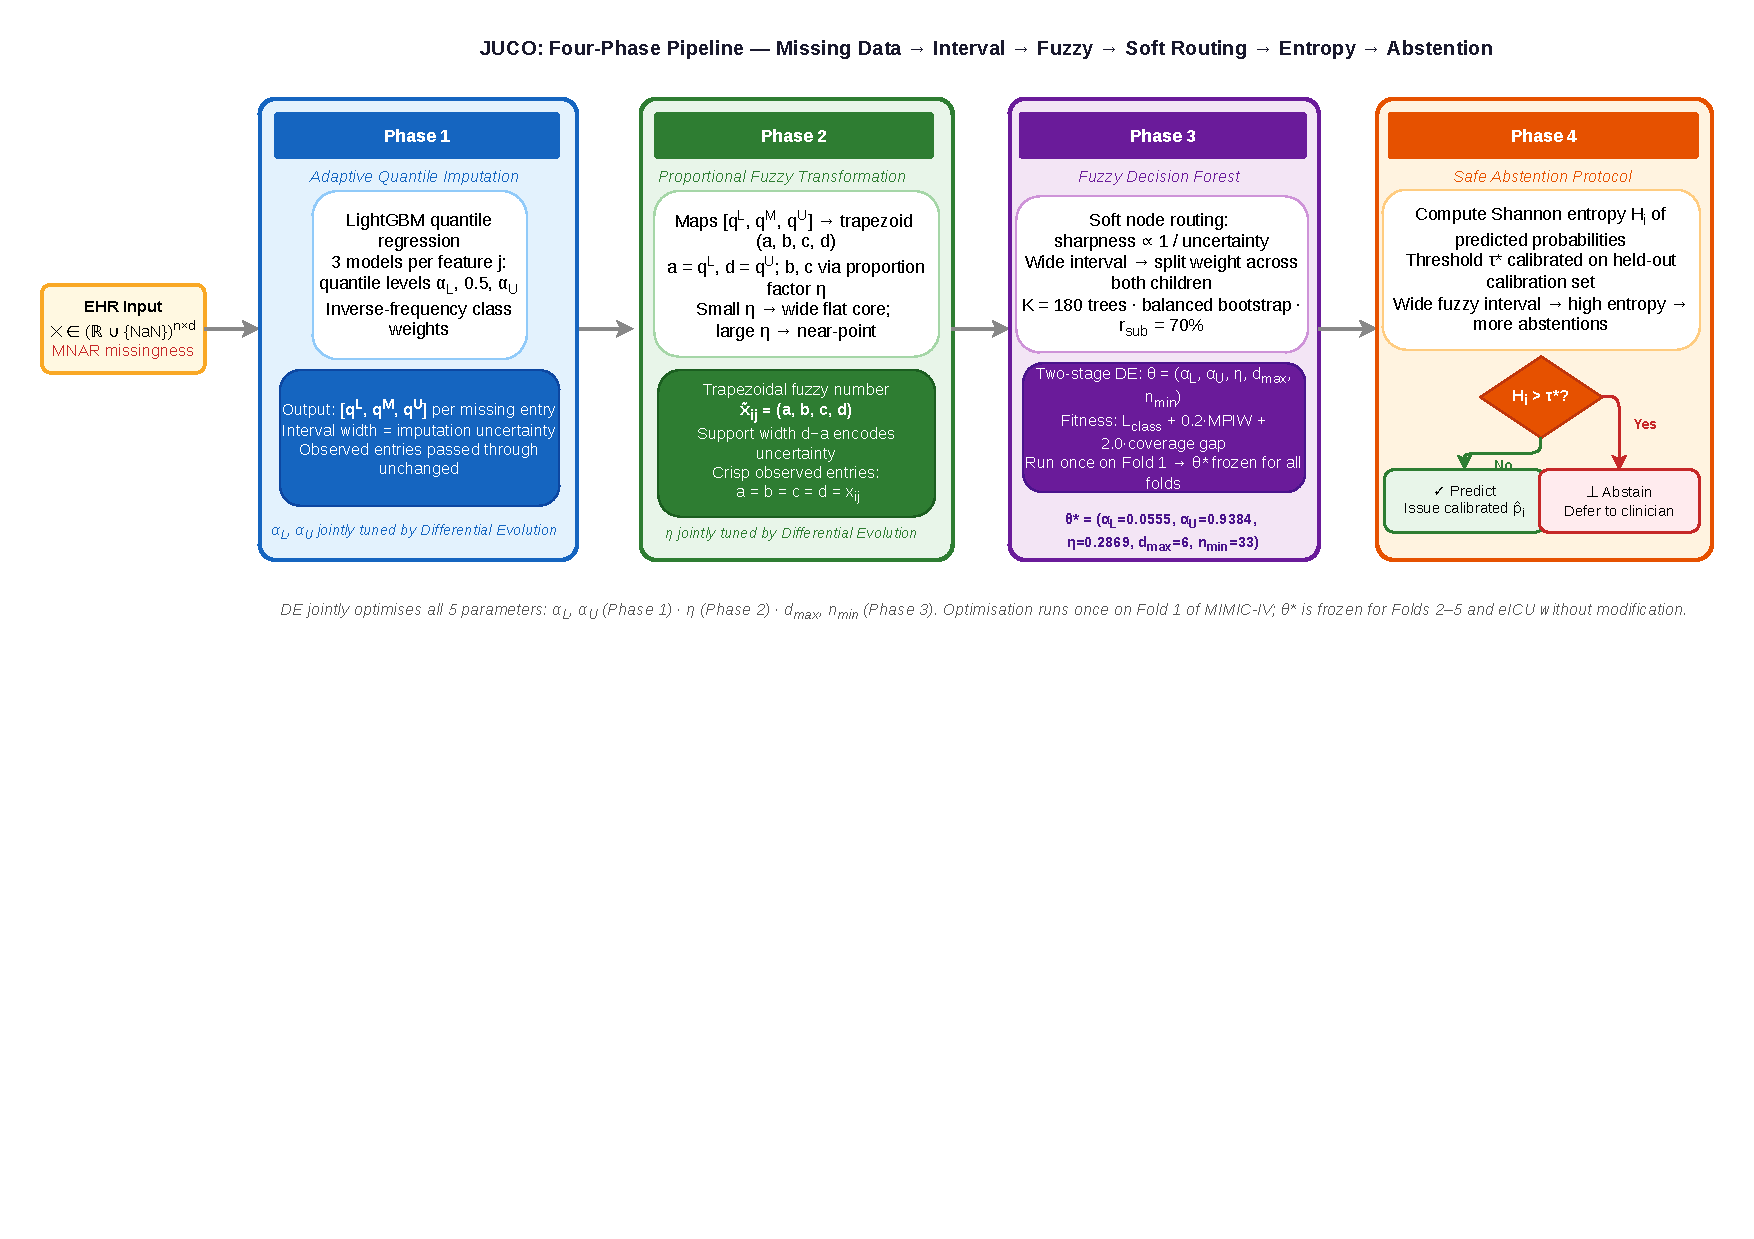
\includegraphics[clip, width=\textwidth]{Figure1.pdf}
		\vspace{-180pt}
		\caption{Overview of the JUCO four-phase pipeline. Phase 1 (Adaptive
			Quantile Imputation) produces prediction intervals $[q^L, q^U]$ for
			each missing entry via LightGBM quantile regression. Phase 2
			(Proportional Fuzzy Transformation) maps these intervals to
			trapezoidal fuzzy numbers $(a,b,c,d)$ whose support width encodes
			imputation uncertainty. Phase 3 (Fuzzy Decision Forest) routes samples
			softly through trees, with uncertain (wide-interval) samples
			distributing their weight across both branches at each node. Phase 4
			(Safe Abstention) calibrates an entropy threshold $\tau$ on a held-out
			calibration set; test samples with $H_i > \tau$ are deferred to
			clinical review.}
		\label{fig:architecture}
	\end{figure}
	
	\subsection{Phase 1: Adaptive Quantile Imputation}
	\label{sec:phase1}
	
	For each feature $j \in \{1, \ldots, d\}$ with missing entries,
	we train a LightGBM quantile regressor to predict the conditional
	quantiles of $x_{ij}$ given the remaining features
	$\mathbf{x}_{i,-j}$.
	The quantile regressor minimises the weighted pinball loss:
	\begin{equation}
		\hat{q}^{\alpha}_{j}(\mathbf{x}_{-j})
		= \arg\min_{f}
		\sum_{i:\, M_{ij}=0}
		w_i \,\rho_{\alpha}\!\left(x_{ij} - f(\mathbf{x}_{i,-j})\right),
		\label{eq:quantile_regression}
	\end{equation}
	where $\rho_{\alpha}(u) = u(\alpha - \mathbf{1}_{u<0})$ is the
	pinball (check) loss at quantile level $\alpha$~\citep{koenker1978regression}, and $w_i$ are
	inverse-frequency sample weights that give rare positive outcomes
	(ICU mortality) equal aggregate influence as the majority class.
	Specifically, the weight assigned to each sample from class~$k$ is:
	\begin{equation}
		w_k = \frac{N}{K \cdot n_k},
		\label{eq:class_weights}
	\end{equation}
	where $N$ is the total number of training samples, $K = 2$ is the
	number of classes, and $n_k$ is the count of class-$k$ samples.
	At $\approx 10\%$ mortality prevalence ($n_1 \approx 0.1N$),
	deceased patients receive approximately ten times the weight of
	surviving patients.
	
	Three regressors are trained per feature at quantile levels
	$\alpha \in \{\alpha_L,\, 0.5,\, \alpha_U\}$, producing for each
	missing entry~$(i,j)$ the triple
	$(q^L_{ij},\, q^M_{ij},\, q^U_{ij})$ representing the lower bound,
	median, and upper bound of the imputed interval.
	The quantile levels $\alpha_L$ and $\alpha_U$ are not fixed;
	they are part of the parameter vector $\boldsymbol{\theta}$
	optimised by Differential Evolution (Section~\ref{sec:de}).
	This allows the framework to adapt the width of imputation
	intervals to the validation loss, rather than pre-specifying a
	fixed confidence level.
	
	For \emph{observed} entries ($M_{ij} = 0$), no imputation is
	performed: the original value $x_{ij}$ is used directly.
	
	\subsection{Phase 2: Proportional Fuzzy Transformation}
	\label{sec:phase2}
	
	Each imputed interval $[q^L_{ij}, q^M_{ij}, q^U_{ij}]$ is mapped to a
	\emph{trapezoidal fuzzy number}~\citep{zimmermann2001fuzzy}
	$\tilde{x}_{ij} = (a_{ij}, b_{ij}, c_{ij}, d_{ij})$
	with membership function:
	\begin{equation}
		\mu_{\tilde{x}_{ij}}(x) =
		\begin{cases}
			0 & x < a_{ij} \text{ or } x > d_{ij}\\
			\dfrac{x - a_{ij}}{b_{ij} - a_{ij}} & a_{ij} \le x < b_{ij}\\
			1 & b_{ij} \le x \le c_{ij}\\
			\dfrac{d_{ij} - x}{d_{ij} - c_{ij}} & c_{ij} < x \le d_{ij}
		\end{cases}
		\label{eq:trapezoid_membership}
	\end{equation}
	The four parameters are constructed from the quantile outputs as:
	\begin{align}
		a_{ij} &= q^L_{ij}, \label{eq:fuzzy_a} \\
		d_{ij} &= q^U_{ij}, \label{eq:fuzzy_d} \\
		b_{ij} &= \max\!\left(a_{ij},\;
		q^M_{ij} - \eta \cdot (q^U_{ij} - q^L_{ij})\right),
		\label{eq:fuzzy_b} \\
		c_{ij} &= \min\!\left(d_{ij},\;
		q^M_{ij} + \eta \cdot (q^U_{ij} - q^L_{ij})\right),
		\label{eq:fuzzy_c}
	\end{align}
	where $\eta \in [0, 0.5]$ is the \emph{proportion factor} that
	controls the ratio of the flat core $[b,c]$ to the total support.
	Small $\eta$ yields a wide flat core (interval-like imputation);
	large $\eta$ yields a peaked trapezoid (near-point imputation).
	For \emph{observed} entries the trapezoid degenerates to a crisp
	value: $a_{ij} = b_{ij} = c_{ij} = d_{ij} = x_{ij}$.
	
	Two derived quantities from the trapezoid are used in the routing
	and optimisation stages:
	\begin{align}
		\text{centroid}(\tilde{x}_{ij}) &= \frac{a_{ij} + b_{ij} + c_{ij} + d_{ij}}{4},
		\label{eq:centroid} \\[4pt]
		\text{uncertainty}(\tilde{x}_{ij}) &= d_{ij} - a_{ij}.
		\label{eq:uncertainty}
	\end{align}
	%% ── FIGURE 2 PLACEHOLDER ─────────────────────────────────────────────────
	%% Location: end of Section 4, before Section 5
	%% Caption:  "Figure 2: Proportional fuzzy transformation.
	%%            Left: Wide quantile interval (high imputation uncertainty)
	%%            produces a broad trapezoid with large support width (d−a).
	%%            Right: Narrow quantile interval (high confidence) produces
	%%            a near-crisp trapezoid.
	%%            The parameter η controls the ratio of the flat core [b,c]
	%%            to the total support [a,d]."
	%% File:     Figure_2.pdf
	%%
	\begin{figure}[htbp]
		\centering
		\vspace{-15pt}
		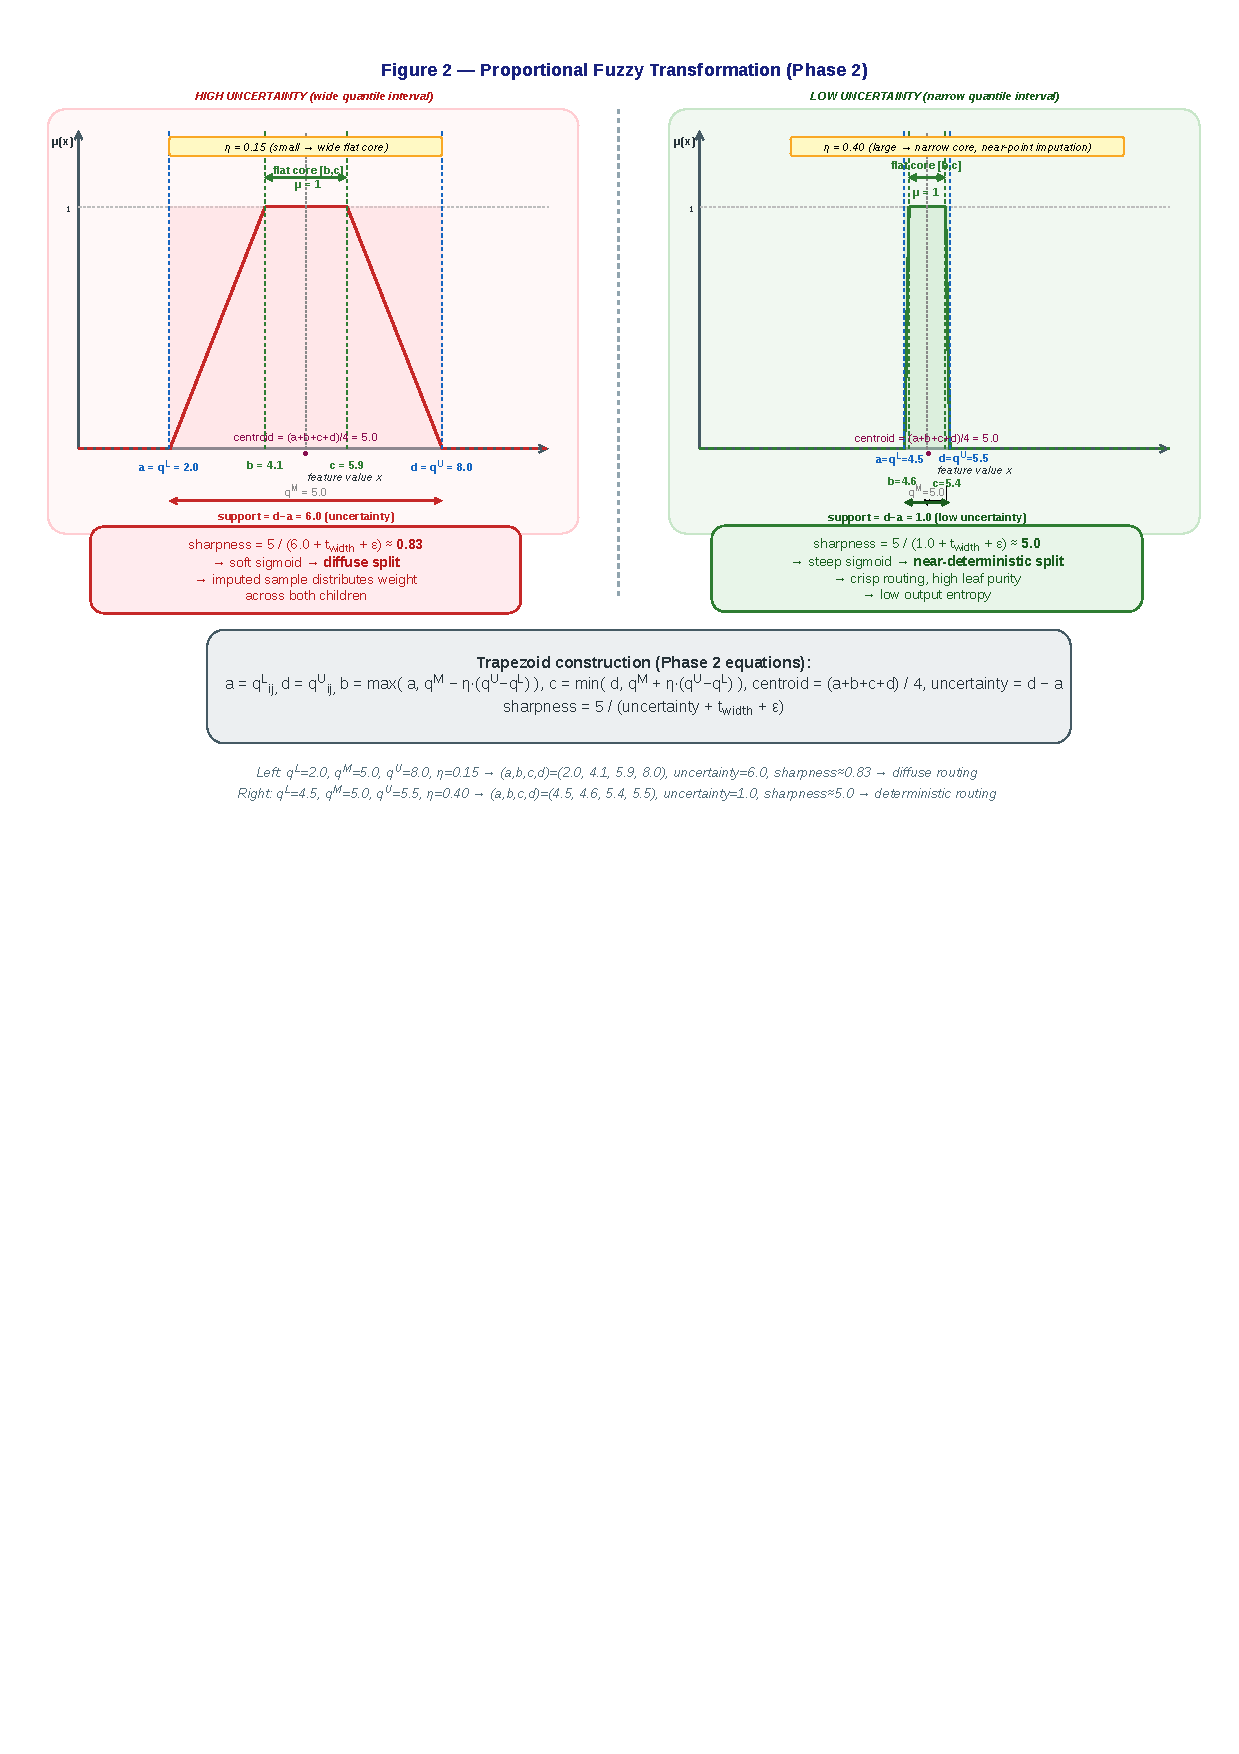
\includegraphics[width=\textwidth]{Figure2.pdf}
		\vspace{-380pt}
		\caption{Proportional fuzzy transformation (Phase 2).
			A missing entry with a wide quantile interval
			$[q^L_{ij}, q^U_{ij}]$ (high imputation uncertainty, left)
			produces a broad trapezoidal fuzzy number with large support
			width $d_{ij} - a_{ij}$, resulting in low sharpness and diffuse
			soft routing at the tree split (Eq.~\ref{eq:sharpness}).
			A narrow interval (high confidence, right) produces a
			near-crisp trapezoid that routes near-deterministically.
			The parameter $\eta$ controls the ratio of the flat core
			$[b_{ij}, c_{ij}]$ to the total support $[a_{ij}, d_{ij}]$.}
		\label{fig:fuzzy_transform}
	\end{figure}

	
	\subsection{Phase 3: Fuzzy Decision Forest}
	\label{sec:phase3}
	
	\subsubsection{Soft Routing at Internal Nodes}
	\label{sec:soft_routing}
	
	Each internal tree node splits samples using soft membership
	degrees rather than hard binary partitions.
	For a node splitting on feature $j$ with threshold
	$\mathcal{T}_t = (t_{\text{center}}, t_{\text{width}})$
	(a triangular fuzzy threshold), the left-child membership
	degree $\mu_{\text{left}} \in [0, 1]$ is computed via a sigmoid
	function whose sharpness adapts inversely to the combined
	uncertainty of the fuzzy number and the threshold:
	\begin{align}
		\text{sharpness}_{ij} &=
		\frac{5}{\text{uncertainty}(\tilde{x}_{ij}) + t_{\text{width}} + \varepsilon},
		\label{eq:sharpness} \\[4pt]
		\mu^L_{ij} &=
		\sigma\!\left(
		\text{sharpness}_{ij} \cdot
		\left(t_{\text{center}} - \text{centroid}(\tilde{x}_{ij})\right)
		\right),
		\label{eq:mu_left} \\[4pt]
		\mu^R_{ij} &= 1 - \mu^L_{ij},
		\label{eq:mu_right}
	\end{align}
	where $\sigma(\cdot)$ is the logistic sigmoid and
	$\varepsilon = 10^{-12}$.
	For observed (crisp) inputs, $d_{ij} = a_{ij}$ so
	uncertainty $= 0$ and $t_{\text{width}} \approx 0$,
	driving sharpness $\to \infty$ and routing to a near-deterministic
	split.
	For imputed inputs with a wide quantile interval,
	$d_{ij} - a_{ij}$ is large, reducing sharpness and distributing
	the sample across both children — naturally down-weighting the
	imputed sample in downstream leaf votes.
	
	\subsubsection{Split Criterion}
	\label{sec:split_criterion}
	
	The best split at each node is chosen to maximise fuzzy
	weighted information gain.
	The \emph{fuzzy weighted entropy} at a node with accumulated
	sample weight vector $\mathbf{w}$ is:
	\begin{equation}
		H_{\text{fuzzy}}(\mathbf{w}, \mathbf{y}) =
		-\sum_{k=0}^{1}
		\tilde{p}_k \log_2(\tilde{p}_k + \varepsilon),
		\quad
		\tilde{p}_k = \frac{\sum_{i:\, y_i = k} w_i}{\sum_i w_i + \varepsilon},
		\label{eq:fuzzy_entropy}
	\end{equation}
	and the \emph{fuzzy information gain} for a candidate split is:
	\begin{equation}
		\Delta H =
		H_{\text{fuzzy}}(\mathbf{w},\, \mathbf{y})
		-
		\frac{\sum_i w_i \mu^L_i}{\sum_i w_i}
		H_{\text{fuzzy}}(\mathbf{w} \circ \boldsymbol{\mu}^L,\, \mathbf{y})
		-
		\frac{\sum_i w_i \mu^R_i}{\sum_i w_i}
		H_{\text{fuzzy}}(\mathbf{w} \circ \boldsymbol{\mu}^R,\, \mathbf{y}),
		\label{eq:fuzzy_ig}
	\end{equation}
	where $\circ$ denotes elementwise multiplication.
	Split thresholds are evaluated at the
	$\{15, 30, 45, 50, 55, 70, 85\}$ percentiles of the centroid
	distribution for each candidate feature.
	
	\subsubsection{Leaf Class Distribution}
	\label{sec:leaf_distribution}
	
	At each leaf node, the class distribution is formed from the
	accumulated soft-routed weight vector $\mathbf{w}^{\ell}$:
	\begin{equation}
		\hat{p}^{\ell}_k
		= \frac{\sum_{i:\, y_i = k} w^{\ell}_i}
		{\sum_i w^{\ell}_i + \varepsilon},
		\quad k \in \{0, 1\}.
		\label{eq:leaf_distribution}
	\end{equation}
	Imputed samples, whose weight is distributed across multiple
	paths, contribute less to any single leaf than observed samples,
	ensuring that uncertainty from Phase 1 influences the leaf
	distribution and hence the final entropy.
	
	\subsubsection{Forest Construction}
	\label{sec:forest}
	
	A \emph{Fuzzy Decision Forest} comprises $K = 180$ trees.
	Each tree is trained on a balanced bootstrap sample: equal numbers
	of positive (mortality) and negative (survival) cases are drawn
	with replacement, counteracting the $\approx 10\%$ class
	prevalence in MIMIC-IV.
	Each tree is assigned a fixed random subset of $\lfloor r_{\text{sub}} \cdot d \rfloor$
	features (with $r_{\text{sub}} = 0.7$), reused for all splits within that tree.
	The final prediction for sample~$i$ is the average class probability
	vector across all $K$ trees:
	\begin{equation}
		\hat{\mathbf{p}}_i = \frac{1}{K} \sum_{k=1}^{K}
		\hat{\mathbf{p}}^{(k)}_i.
		\label{eq:forest_prediction}
	\end{equation}
	Isotonic calibration~\citep{zadrozny2002transforming} is applied
	post-hoc on a held-out calibration set.
	
	\subsubsection{Two-Stage Differential Evolution}
	\label{sec:de}
	
	Differential Evolution (DE)~\citep{storn1997differential} is a
	population-based global optimiser well suited to mixed
	continuous/integer search spaces with non-differentiable fitness
	functions.
	The five-dimensional parameter vector
	$\boldsymbol{\theta} = (\alpha_L, \alpha_U, \eta, d_{\max},
	n_{\min})$ is optimised jointly across all four phases.
	The search bounds are:
	\begin{equation}
		\boldsymbol{\theta} \in
		[0.05, 0.35] \times [0.65, 0.95] \times [0.1, 0.5]
		\times [4, 6] \times [15, 50].
		\label{eq:de_bounds}
	\end{equation}
	The composite fitness function to be minimised is:
	\begin{equation}
		\mathcal{L}(\boldsymbol{\theta})
		= L_{\text{class}}
		+ \lambda_1 \cdot \text{MPIW}_{\text{norm}}
		+ \lambda_2 \cdot \text{coverage\_gap},
		\label{eq:composite_fitness}
	\end{equation}
	where $L_{\text{class}}$ is log-loss on the validation set,
	$\text{MPIW}_{\text{norm}}$ is the normalised Mean Prediction
	Interval Width (penalising overly wide intervals):
	\begin{equation}
		\text{MPIW}_{\text{norm}} =
		\frac{1}{d} \sum_{j=1}^{d}
		\frac{\overline{|q^U_j - q^L_j|}}{\max_j - \min_j + \varepsilon},
		\label{eq:mpiw}
	\end{equation}
	and $\text{coverage\_gap}$ penalises intervals that fail to cover
	the true values at the 95\% target level:
	\begin{equation}
		\text{coverage\_gap} =
		\max\!\left(0,\; 0.95 - \widehat{\text{PICP}}\right),
		\label{eq:coverage_gap}
	\end{equation}
	where $\widehat{\text{PICP}}$ (Prediction Interval Coverage
	Probability) is the empirical fraction of masked true values
	falling within $[q^L, q^U]$:
	\begin{equation}
		\widehat{\text{PICP}} =
		\frac{1}{|\mathcal{M}|}
		\sum_{(i,j)\in\mathcal{M}}
		\mathbf{1}\!\left[q^L_{ij} \le x^{\text{true}}_{ij} \le q^U_{ij}\right],
		\label{eq:picp}
	\end{equation}
	with $\mathcal{M}$ the set of artificially masked entries for which
	the ground-truth value is available.
	The penalty weights are $\lambda_1 = 0.2$ and $\lambda_2 = 2.0$.
	
	\textbf{Two-stage schedule.}
	Stage 1 uses a proxy forest ($K = 20$ trees, 2{,}000
	subsampled training points) for a fast global search.
	Stage 2 seeds the population around the Stage-1 optimum and
	evaluates with a larger proxy ($K = 40$ trees, up to 7{,}000 points)
	for accurate local refinement.
	DE is run \emph{once on Fold~1} of MIMIC-IV; the resulting
	$\boldsymbol{\theta}^*$ is frozen and applied to all subsequent folds
	and to eICU without modification.
	
	\subsection{Phase 4: Safe Abstention Protocol}
	\label{sec:phase4}
	
	The Shannon entropy of the predicted class probability vector is:
	\begin{equation}
		H_i = -\sum_{k} \hat{p}_{ik} \ln(\hat{p}_{ik} + \varepsilon).
		\label{eq:entropy}
	\end{equation}
	An entropy threshold $\tau$ is calibrated on the held-out
	calibration set by finding the largest prefix (sorted by
	increasing $H$) whose cumulative error rate does not exceed
	$\epsilon_{\max} = 5\%$:
	\begin{equation}
		\tau^* = \max\!\left\{
		H_{(\ell)} :
		1 - \frac{1}{\ell}\sum_{i=1}^{\ell} \mathbf{1}[\hat{y}_i = y_i]
		\le \epsilon_{\max}
		\right\},
		\label{eq:tau_calibration}
	\end{equation}
	where $H_{(1)} \le H_{(2)} \le \cdots$ are the sorted entropies.
	Any test sample with $H_i > \tau^*$ is flagged as \emph{abstained}
	and deferred to clinical review; the remainder receive the
	calibrated risk estimate $\hat{p}_i$.
	
	Performance under selective prediction is evaluated via the AURC:
	\begin{equation}
		\text{AURC} = \int_0^1 r(\kappa)\, \mathrm{d}\kappa
		\approx \sum_{i} r_i \cdot \Delta\kappa_i,
		\label{eq:aurc}
	\end{equation}
	where $\kappa$ is coverage (fraction of samples predicted)
	and $r(\kappa)$ is the error rate on the most confident
	$100\kappa\%$ of predictions.
	
	\subsection{MNAR Stress Test Design}
	\label{sec:mnar_stress}
	
	To measure robustness to distributional shift in the missingness
	mechanism, additional synthetic missingness is applied at test time
	only, using a logistic dropout model~\citep{sterne2009multiple,
		josse2019consistency}:
	\begin{equation}
		P(M_{ij} = 1 \mid x_{ij}) =
		\sigma\!\left(\beta \cdot \tilde{x}_{ij} + \gamma\right),
		\label{eq:mnar_mask}
	\end{equation}
	where $\tilde{x}_{ij}$ is the min-max normalised value of feature~$j$,
	$\beta = -1.0$, and $\gamma = 0.0$ throughout this study.
	With $\beta < 0$, higher-valued features are \emph{less} likely to
	be masked, mimicking the clinical pattern where abnormal laboratory
	results are more likely to be recorded.
	
	\subsection{JUCO-XGB Ablation Variant}
	\label{sec:juco_xgb}
	
	To assess whether the fuzzy forest backbone is necessary, a variant
	\textbf{JUCO-XGB} replaces the fuzzy forest with an XGBoost classifier
	trained on interval-valued features $[q^L_{ij}, q^M_{ij}, q^U_{ij}]$
	directly (six inputs per original feature: three quantiles for each
	of two relevant features).
	JUCO-XGB uses the same DE-optimised imputation parameters
	$(\alpha_L^*, \alpha_U^*)$ but does not perform fuzzy transformation
	or soft routing.
	Comparison between JUCO and JUCO-XGB isolates the contribution of
	the fuzzy forest independently of imputation quality.
	
	
	
	%% ──────────────────────────────────────────────────────────────────────────
	
	
	%% =========================================================================
	%%  SECTION 5 — EXPERIMENTAL SETUP (body from verified sec5 file)
	%% =========================================================================
	
	\section{Experimental Setup}
	\label{sec:experimental_setup}
	
	\subsection{Datasets}
	\label{sec:datasets}
	
	\paragraph{MIMIC-IV (primary cohort).}
	The Medical Information Mart for Intensive Care version
	IV~\citep{johnson2023mimic} is a publicly available, single-centre
	EHR database from Beth Israel Deaconess Medical Center (Boston, MA).
	We extracted all adult ICU admissions (age $\ge 18$), excluding
	admissions shorter than 4 hours or longer than 30 days.
	All clinical variables were aggregated over the first 24 hours of
	ICU admission, consistent with standard ICU mortality prediction
	literature~\citep{purushotham2018benchmarking}.
	The primary outcome is in-hospital mortality (binary).
	After preprocessing and feature selection (Section~\ref{sec:feature_selection}),
	the cohort comprises 82{,}785 stays with
	10.58\% mortality prevalence.
	
	\paragraph{eICU (external validation).}
	The eICU Collaborative Research Database~\citep{pollard2018eicu}
	contains data from 208 US hospitals with 162{,}136
	ICU admissions.
	It was used exclusively for external validation with no re-training
	or re-optimisation: JUCO parameters frozen from MIMIC-IV Fold~1 DE
	were applied directly.
	This design tests cross-institutional generalisation under genuine
	distribution shift in patient demographics, hospital protocols,
	and missingness patterns.
	
	\subsection{Feature Selection}
	\label{sec:feature_selection}
	
	Mutual information (MI) between each feature and the mortality label
	was computed on the training fold only.
	The top 35 features (of $\approx$80 candidate features) were retained.
	This conservative selection was imposed by the computational
	requirements of two-stage DE optimisation.
	
	\subsection{Evaluation Protocol}
	\label{sec:evaluation_protocol}
	
	All MIMIC-IV evaluations use stratified 5-fold
	GroupKFold cross-validation at the \emph{patient level}, ensuring
	that no two ICU stays from the same patient appear in both training
	and test partitions.
	The training fold is further split into
	train (60\%) / validation (20\%) / calibration (20\%) subsets
	at the patient level.
	The \emph{validation} subset is used by DE fitness evaluation.
	The \emph{calibration} subset is used for post-hoc isotonic
	calibration and abstention threshold calibration (Section~\ref{sec:phase4}).
	DE hyperparameter search was conducted on Fold~1 only;
	the resulting $\boldsymbol{\theta}^*$ was applied to Folds~2--5 and
	eICU without modification.
	
	MNAR augmentation (Eq.~\ref{eq:mnar_mask}, target rate 30\%)
	was applied only to training and validation folds.
	Test sets and eICU retain their natural missingness.
		%% ── FIGURE 3 PLACEHOLDER ─────────────────────────────────────────────────
	%% Location: end of Section 5 (or start of Section 6 Results)
	%% Caption:  "Figure 3: Evaluation protocol diagram.
	%%            Patient-level GroupKFold 5-fold CV on MIMIC-IV.
	%%            Each fold splits into Train (60%) / Validation (20%) /
	%%            Calibration (20%). DE runs on Fold 1 only. Frozen θ*
	%%            applied to Folds 2–5 and eICU. MNAR augmentation applied
	%%            only to train/val; test and eICU use natural missingness."
	%% File:     Figure_3.pdf
	%%
	\begin{figure}[!htbp]
		\centering
			\vspace{-10pt}
		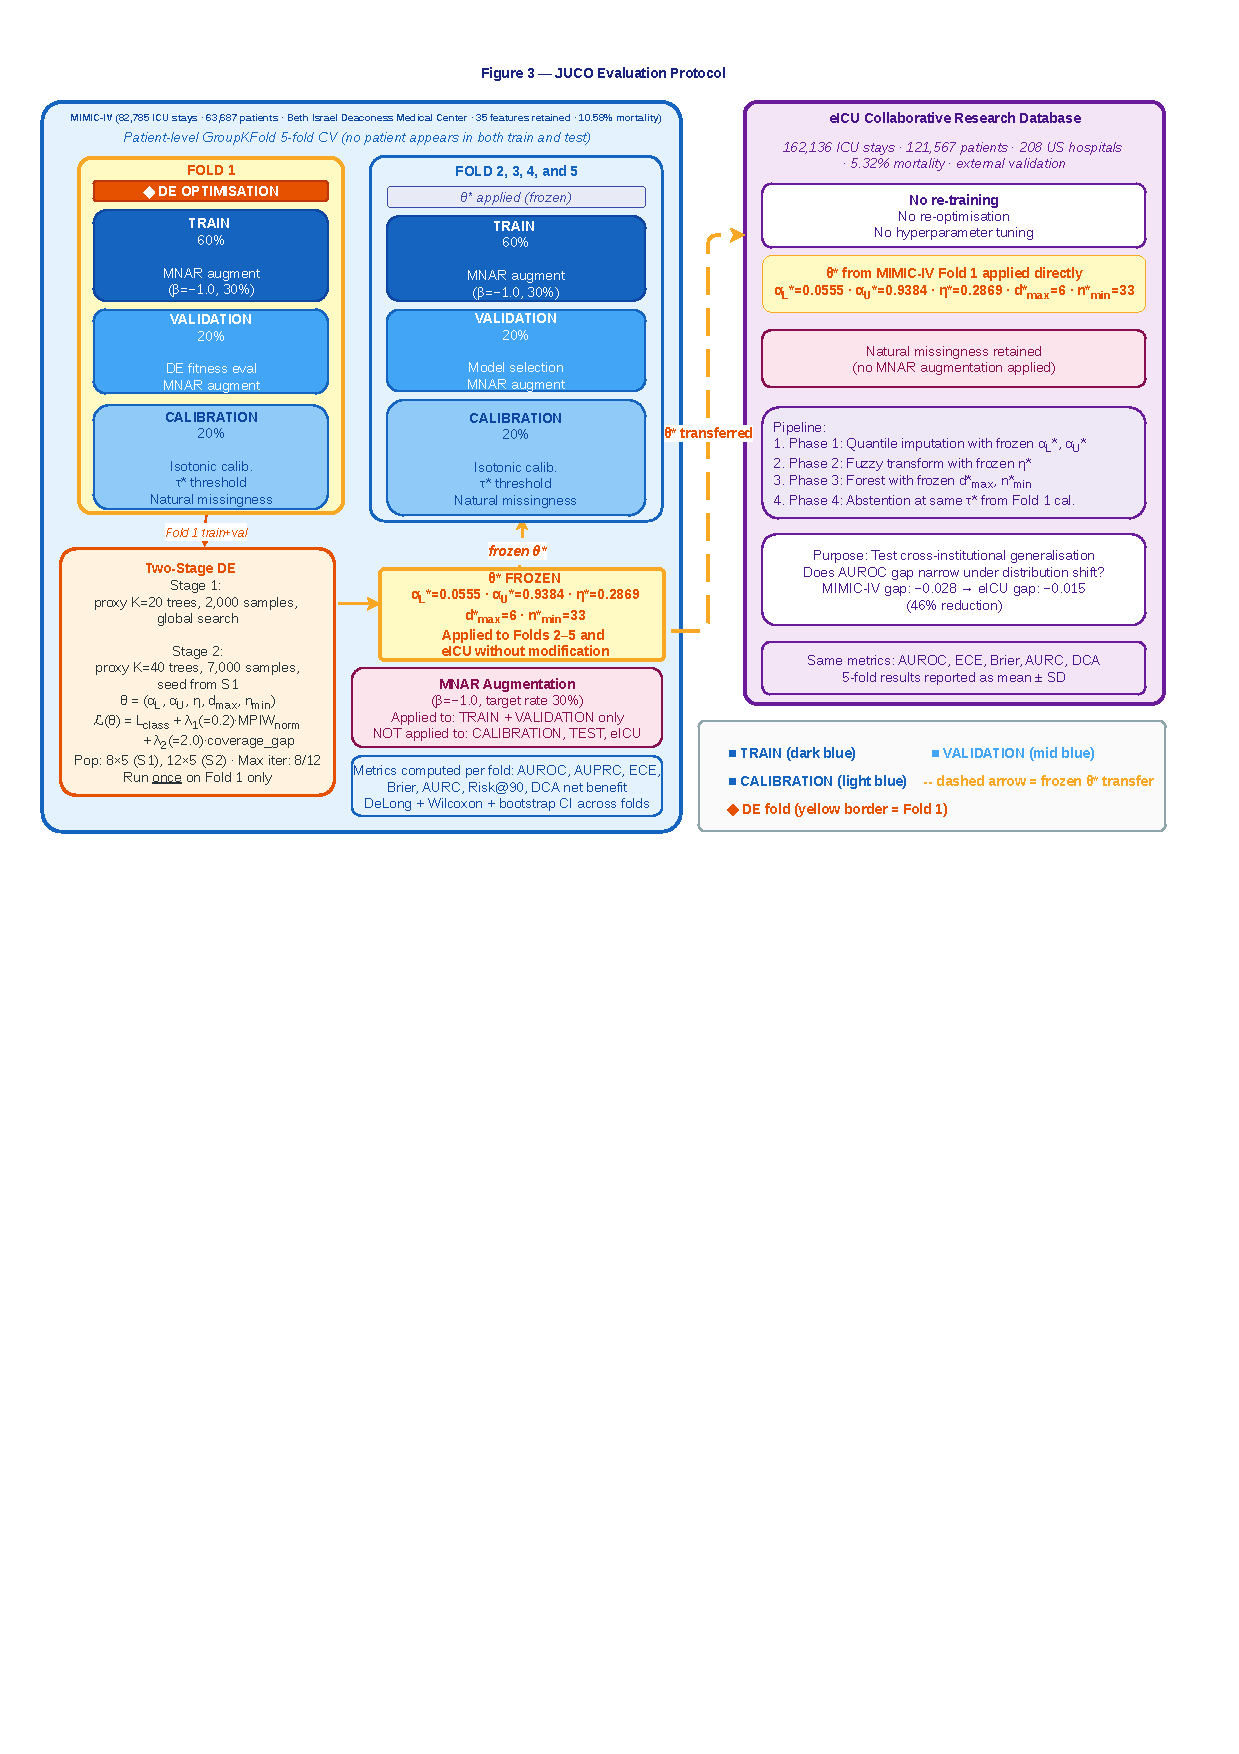
\includegraphics[width=\linewidth]{Figure3.pdf}
		\vspace{-330pt}
		\caption{Evaluation protocol. MIMIC-IV is partitioned using
			patient-level GroupKFold 5-fold cross-validation to prevent
			data leakage. Each training fold is further divided into train,
			validation, and calibration subsets.
			DE hyperparameter search runs once on Fold~1;
			the resulting $\boldsymbol{\theta}^*$ is frozen and applied
			unchanged to Folds~2--5 and the eICU external validation set.
			MNAR augmentation (Eq.~\ref{eq:mnar_mask}) is applied only to
			training and validation subsets.}
		
		\label{fig:eval_protocol}
	\end{figure}

	
	\subsection{Post-Hoc Calibration}
	\label{sec:calibration}
	
	All model outputs are post-hoc calibrated using isotonic regression
	fitted on the calibration set.
	Isotonic calibration is preferred over Platt scaling for
	tree-based models because it is non-parametric and does not
	assume a sigmoid relationship between raw scores and
	probabilities~\citep{zadrozny2002transforming}.
	The calibrated probabilities are used for all metric computation,
	DCA, and abstention threshold calibration.
	All baselines undergo the same calibration procedure.
	
	\subsection{Baselines}
	\label{sec:baselines}
	
	The following baselines are evaluated under identical preprocessing,
	feature selection, and calibration procedures:
	\textbf{XGBoost}~\citep{chen2016xgboost} and
	\textbf{LightGBM}~\citep{ke2017lightgbm}
	with native NaN routing (no imputation);
	\textbf{MissForest+XGB}: MissForest imputation~\citep{stekhoven2012missforest}
	followed by XGBoost;
	\textbf{MeanImp+XGB}: mean imputation followed by XGBoost;
	\textbf{TabNet}~\citep{arik2021tabnet}: a deep learning model
	with attention-based feature selection, included as a DL baseline;
	\textbf{JUCO-XGB}: the ablation variant described in Section~\ref{sec:juco_xgb}.
	
	\subsection{Evaluation Metrics}
	\label{sec:metrics}
	
	\paragraph{Discrimination.}
	\emph{AUROC} (Area Under the Receiver Operating Characteristic
	Curve) is the primary metric.
	\emph{AUPRC} (Area Under the Precision-Recall Curve) is reported
	as a secondary metric more informative than AUROC for class-imbalanced
	outcomes.
	
	\paragraph{Calibration.}
	\emph{Expected Calibration Error} (ECE) measures the
	sample-weighted mean absolute deviation between predicted
	probabilities and empirical outcome frequencies across 15
	equal-width bins~\citep{naeini2015obtaining}:
	\begin{equation}
		\text{ECE} = \sum_{b=1}^{B} \frac{n_b}{N}
			\left|\overline{p}_b - \text{freq}_b\right|, \quad B = 15,
		\label{eq:ece}
	\end{equation}
	where $\overline{p}_b$ is the mean predicted probability in bin~$b$,
	$\text{freq}_b$ is the fraction of positive outcomes in that bin,
	$n_b$ is the number of samples in bin~$b$, and $N$ is the total
	number of samples.
	
	The \emph{Brier Score}~\citep{brier1950verification} measures
	mean-squared error between predicted probabilities and labels:
	\begin{equation}
		\text{BS} = \frac{1}{n}\sum_{i=1}^{n}(\hat{p}_i - y_i)^2.
		\label{eq:brier}
	\end{equation}
	
	\paragraph{Selective prediction.}
	\emph{AURC} (Eq.~\ref{eq:aurc}) quantifies how effectively a model
	concentrates errors in the high-entropy (abstained) region.
	\emph{Risk@90} is the error rate on the most confident 90\% of
	predictions, representing the scenario where 10\% of cases are
	deferred to clinician review.
	
	\paragraph{Clinical utility.}
	\emph{Decision Curve Analysis} (DCA)~\citep{vickers2006decision}
	computes the net benefit of each model relative to treat-all and
	treat-none strategies:
	\begin{equation}
		\text{NB}(p_t) =
		\frac{\text{TP}}{n} - \frac{p_t}{1 - p_t} \cdot \frac{\text{FP}}{n},
		\label{eq:net_benefit}
	\end{equation}
	where $p_t \in [0.01, 0.49]$ is the clinical decision threshold.
	
	\subsection{Statistical Tests}
	\label{sec:statistical_tests}
	
	\paragraph{Wilcoxon signed-rank test (fold-level).}
	A paired Wilcoxon signed-rank test~\citep{wilcoxon1945individual}
	was applied to the five per-fold AUROC values for each JUCO vs
	baseline comparison.
	With only 5 folds, the minimum achievable two-sided Wilcoxon
	$p$-value is $p = 0.0625$; no comparison reached formal significance.
	
	\paragraph{DeLong test (patient-level).}
	DeLong's method~\citep{delong1988comparing} was applied to
	the pooled patient-level predictions within each dataset.
	This test is adequately powered given the large sample sizes
	($n = 82{,}785$ MIMIC-IV, $n = 162{,}136$ eICU).
	All DeLong $p$-values are reported transparently, including those
	indicating JUCO's statistically inferior AUROC relative to gradient
	boosting under standard conditions.
	A Bonferroni correction for four simultaneous comparisons per
	dataset sets the significance threshold at $\alpha = 0.0125$.
	
	\paragraph{Bootstrap confidence intervals.}
	Stratified bootstrap confidence intervals (1{,}000 resamples,
	$\alpha = 0.05$) were computed for AUROC on both datasets.

	\subsection{Computational Environment and Complexity}
	\label{sec:compute}

	\paragraph{Hardware and software.}
	All experiments were executed on Google Cloud Platform (GCP)
	using a \texttt{n2-standard-32} virtual machine instance
	(32 vCPUs, 128\,GB RAM).
	The software stack comprised \texttt{Python},
	\texttt{scikit-learn}, \texttt{LightGBM},
	\texttt{SciPy} (for \texttt{differential\_evolution}),
	\texttt{joblib}, \texttt{NumPy}, and
	\texttt{DuckDB} for streaming eICU data.
	No GPU acceleration was used; all computation is CPU-bound.
	Parallelism was exploited at two levels: the DE population
	was evaluated with 12 parallel workers
	(\texttt{de\_workers}$=12$, \texttt{updating="deferred"}),
	and the full 180-tree forest was built using 28 \texttt{joblib}
	workers (\texttt{forest\_workers}$=28$, \texttt{backend="loky"}).

	\paragraph{Time complexity.}
	Let $n$ denote training set size, $d = 35$ selected features,
	$B = 50$ boosting rounds (Phase~1),
	$K = 180$ fuzzy trees (Phase~3), $D_{\max} = 6$ maximum depth,
	and $r_{\text{sub}} = 0.7$ so that $d_{\text{sub}} =
	\lfloor r_{\text{sub}} \cdot d \rfloor = 24$ features per tree.

	\begin{itemize}[nosep, leftmargin=*]
		\item \textbf{Phase~1} (Adaptive Quantile Imputation):
		      $O(n \cdot d \cdot B \cdot \log n)$ — one LightGBM
		      quantile imputer trained per fold.

		\item \textbf{Phase~2} (Fuzzy Transformation):
		      $O(n \cdot d)$ — fully vectorised, negligible cost.

		\item \textbf{Phase~3 — Forest training}:
		      $O\!\left(K \cdot n \cdot d_{\text{sub}} \cdot
		      D_{\max}\right)$, parallelised over $K$ trees.

		\item \textbf{Phase~3 — DE optimisation} (one-time, Fold~1 only):
		      $O\!\left(G \cdot P \cdot
		      K_{\text{proxy}} \cdot n_{\text{proxy}} \cdot
		      d_{\text{sub}} \cdot D_{\max}\right)$,
		      where Stage~1 uses $G_1 \le 8$ generations,
		      $P_1 = 8 \times 5 = 40$ candidates,
		      $K_{\text{proxy}}^{(1)} = 20$ trees, and
		      $n_{\text{proxy}}^{(1)} = 2{,}000$ samples;
		      Stage~2 uses $G_2 \le 12$, $P_2 = 60$,
		      $K_{\text{proxy}}^{(2)} = 40$, and
		      $n_{\text{proxy}}^{(2)} = 7{,}000$.
		      Total proxy evaluations: ${\le}1{,}040$, parallelised over 12 workers.

		\item \textbf{Phase~4} (Abstention thresholding):
		      $O(n_{\text{cal}} \log n_{\text{cal}})$ — entropy sort
		      on the calibration subset, negligible cost.
	\end{itemize}

	The per-fold complexity is
	$O\!\left(n \cdot d \cdot (B \log n + K \cdot D_{\max})\right)$,
	scaling \emph{linearly} in $n$ and $d$.

	\paragraph{Wall-clock runtimes.}
	Table~\ref{tab:runtimes} summarises wall-clock times on the
	GCP \texttt{n2-standard-32} instance.
	\FloatBarrier
	\begin{table}[ht]
		\centering
		\caption{Wall-clock runtimes on GCP \texttt{n2-standard-32}
			(32 vCPUs, 128\,GB RAM).
			MIMIC-IV Fold~1 includes two-stage DE optimisation;
			Folds~2--5 reuse the frozen $\boldsymbol{\theta}^*$.
			eICU timings are measured from the run log.}
		\label{tab:runtimes}
		\small
		\begin{tabular}{llr}
			\toprule
			\textbf{Pipeline} & \textbf{Stage} & \textbf{Time (min)} \\
			\midrule
			MIMIC-IV & DE Stage~1 (coarse search) & $\approx$20 \\
			         & DE Stage~2 (fine refinement) & $\approx$50 \\
			         & Fold~1 (DE + fold training) & $\approx$85 \\
			         & Folds~2--5 (frozen $\boldsymbol{\theta}^*$, each) & $\approx$15 \\
			         & \textit{Total (all 5 folds)} & $\approx$145 \\
			\midrule
			eICU     & Fold~1 & 21.8 \\
			         & Fold~2 & 22.2 \\
			         & Fold~3 & 22.0 \\
			         & Fold~4 & 23.7 \\
			         & Fold~5 & 23.5 \\
			         & \textit{Total (all 5 folds)} & 113.7 \\
			\bottomrule
		\end{tabular}
	\end{table}
	\FloatBarrier
	MIMIC-IV Folds~2--5 each take approximately 15 minutes
	(frozen parameters, no DE).
	Fold~1 is substantially longer due to the two-stage DE search:
	Stage~1 (up to $8 \times 40 = 320$ candidate evaluations on a
	lightweight proxy) took $\approx$20 minutes, and Stage~2
	(up to $12 \times 60 = 720$ evaluations on a larger proxy)
	took $\approx$50 minutes, for a total DE overhead of
	$\approx$70 minutes on top of the 15-minute fold training.
	The original MIMIC-IV live log was not retained;
	eICU timings are measured directly from the GCP run log.



	%% ──────────────────────────────────────────────────────────────────────────
	
	
	%% =========================================================================
	%%  SECTION 6 — RESULTS
	%% =========================================================================
	\clearpage
	\section{Results}
	\label{sec:results}
	
	We present results in the order of the evaluation objectives
	defined in Section~\ref{sec:eval_objectives}: robustness under
	missingness shift, safe abstention quality, cross-institutional
	generalisation, baseline comparison under standard conditions,
	and decision curve analysis.
	
	\subsection{Robustness Under Escalating MNAR Missingness}
	\label{sec:stress_results}
	\FloatBarrier
	%% ── FIGURE 4 PLACEHOLDER ──────────────────────────────────────────────────
	%% Location: immediately before Table 1 (or after it)
	%% Caption:  "Figure 4: AUROC vs MNAR missingness rate (10%–70%).
	%%            JUCO (solid blue), XGBoost (dashed orange), LightGBM
	%%            (dotted green), MissForest+XGB (dash-dot red), MeanImp+XGB
	%%            (dashed purple). Error bars show ±1 SD across 2 folds.
	%%            At 70% JUCO overtakes XGBoost and MissForest+XGB.
	%%            LightGBM remains above JUCO throughout (discussed in §7.2)."
	%% File:     Figure_4.pdf
	%%
	\begin{figure}[h]
		\centering
	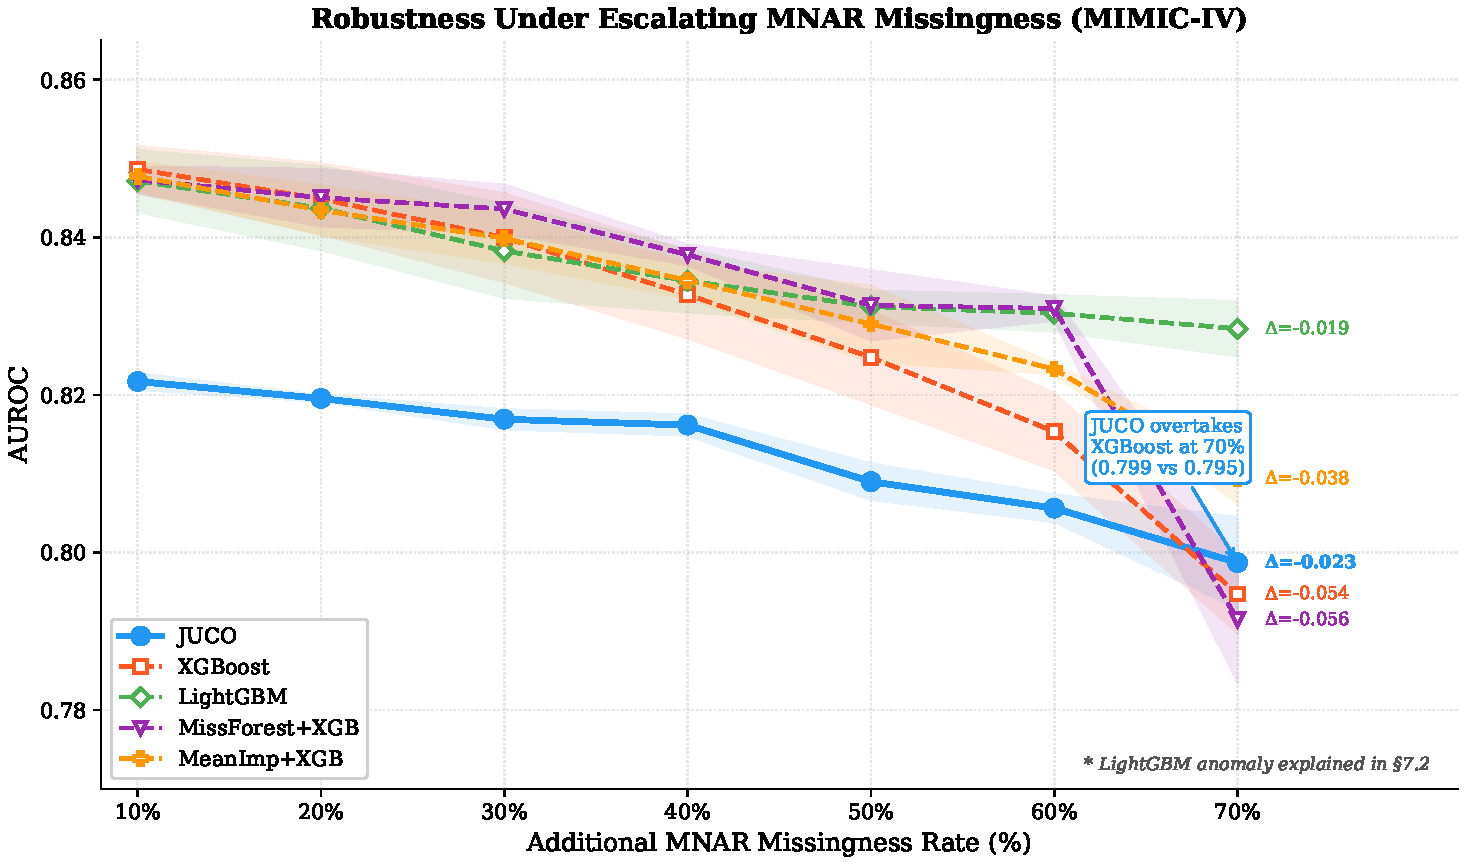
\includegraphics[width=\linewidth]{Figure4.pdf}
		\caption{AUROC as a function of additional MNAR missingness rate
			(10\%--70\%) on MIMIC-IV, evaluated on 2 folds.
			JUCO's degradation ($-0.023$) is substantially smaller than
			XGBoost ($-0.054$) and MissForest+XGB ($-0.056$).
			JUCO overtakes both models at 70\% missingness.
			LightGBM's anomalous robustness ($-0.019$) is explained
			mechanistically in Section~\ref{sec:lightgbm_anomaly}.
			Error bars show $\pm 1$ SD across the two evaluation folds.}
		\label{fig:stress_test}
	\end{figure}

	%% ──────────────────────────────────────────────────────────────────────────
	\vspace{20pt}
	Table~\ref{tab:stress_test} presents AUROC for all models across
	seven MNAR rates (10\%--70\%).
	At 10\% missingness, gradient boosting methods achieve higher
	AUROC (XGBoost 0.849, LightGBM 0.847, MissForest+XGB 0.847,
	MeanImp+XGB 0.848) than JUCO (0.822), consistent with their
	advantage under in-distribution conditions.
	As missingness increases, gradient boosting degrades substantially:
	at 70\%, XGBoost reaches 0.795 ($\Delta = -0.054$) and
	MissForest+XGB reaches 0.792 ($\Delta = -0.056$).
	JUCO's degradation is $-0.023$ (0.822 $\to$ 0.799), and at 70\%
	JUCO overtakes both XGBoost and MissForest+XGB.
	MeanImp+XGB shows intermediate robustness ($\Delta = -0.038$,
	reaching 0.809 at 70\%).
	LightGBM is the anomalous case, degrading by only $-0.019$
	(0.847 $\to$ 0.828) and remaining above JUCO at all rates;
	this is explained in Section~\ref{sec:lightgbm_anomaly}.
	
	\begin{table}[h]
		\centering
		\caption{AUROC under escalating MNAR missingness (MIMIC-IV, 2 folds,
			mean $\pm$ SD). Bold: highest AUROC at each rate.
			$\dagger$: JUCO outperforms gradient boosting at this rate.}
		\label{tab:stress_test}
		\small
		\resizebox{\linewidth}{!}{%
			\begin{tabular}{lccccccc}
				\toprule
				\textbf{Model} & \textbf{10\%} & \textbf{20\%} & \textbf{30\%} &
				\textbf{40\%} & \textbf{50\%} & \textbf{60\%} & \textbf{70\%} \\
				\midrule
				JUCO (Ours)         & 0.822 & 0.820 & 0.817 & 0.816 & 0.809 & 0.806 & 0.799$\dagger$ \\
				XGBoost             & \textbf{0.849} & \textbf{0.845} & 0.840 & 0.833 & 0.825 & 0.815 & 0.795 \\
				LightGBM            & 0.847 & 0.844 & 0.838 & 0.835 & \textbf{0.831} & 0.830 & \textbf{0.828} \\
				MissForest+XGB      & 0.847 & \textbf{0.845} & \textbf{0.844} & \textbf{0.838} & \textbf{0.831} & \textbf{0.831} & 0.792$\dagger$ \\
				MeanImp+XGB         & 0.848 & 0.843 & 0.840 & 0.835 & 0.829 & 0.823 & 0.809 \\
				\midrule
				$\Delta$ JUCO       & ---   &       & $-0.005$ &      &       &       & $-0.023$ \\
				$\Delta$ XGBoost    & ---   &       & $-0.009$ &      &       &       & $-0.054$ \\
				$\Delta$ MissForest & ---   &       & $-0.004$ &      &       &       & $-0.056$ \\
				\bottomrule
		\end{tabular}}
	\end{table}
	\FloatBarrier
	
	\subsection{Ablation Study: Component Contributions}
	\label{sec:ablation_results}
	
	Table~\ref{tab:ablation} presents results for six architectural
	variants evaluated on 2 MIMIC-IV folds.
	\vspace{5pt}
	\begin{table}[h]
		\centering
		\caption{Ablation study results (MIMIC-IV, 2 folds, mean $\pm$ SD).
			Bold: best ablation variant per metric (JUCO Full shown as reference).
			The largest single-component contribution is safe abstention
			(A4 AURC: 0.0895 vs Full: 0.0319, a $2.8{\times}$ increase without
			abstention). ECE values for JUCO Full and A4 are reported from the
			5-fold main evaluation (Table~\ref{tab:main_results}) for consistency;
			the 2-fold ablation run yields ECE $= 0.0049$ for both variants.}
		\vspace{5pt}
		\label{tab:ablation}
		\small
		\begin{tabular}{lcccc}
			\toprule
			\textbf{Variant} & \textbf{AUROC} & \textbf{ECE} & \textbf{Brier} & \textbf{AURC} \\
			\midrule
			JUCO (Full)       & 0.818 $\pm$ 0.001          & 0.0063 $\pm$ 0.0016          & 0.072 $\pm$ 0.000          & 0.0319 $\pm$ 0.0010 \\
			A1: Sequential    & 0.820 $\pm$ 0.003          & \textbf{0.0034} $\pm$ 0.0019 & \textbf{0.070} $\pm$ 0.000 & 0.0324 $\pm$ 0.0008 \\
			A2: Crisp Forest  & 0.811 $\pm$ 0.004          & 0.0071 $\pm$ 0.0006          & 0.071 $\pm$ 0.001          & 0.0349 $\pm$ ${<}$0.0001 \\
			A3: Point Impute  & 0.819 $\pm$ 0.000          & 0.0053 $\pm$ 0.0012          & 0.072 $\pm$ 0.001          & 0.0320 $\pm$ 0.0007 \\
			A4: No Abstention & 0.818 $\pm$ 0.001          & 0.0063 $\pm$ 0.0016          & 0.072 $\pm$ 0.000          & 0.0895$^{\dagger}$ $\pm$ 0.0005 \\
			A5: No MNAR Aug   & \textbf{0.821} $\pm$ 0.002 & 0.0043 $\pm$ 0.0010          & 0.072 $\pm$ 0.000          & \textbf{0.0314} $\pm$ 0.0014 \\
			\bottomrule
		\end{tabular}
		\par\smallskip
		\raggedright\footnotesize
		$^{\dagger}$A4 makes no abstentions; the risk--coverage curve is
		flat at the full-coverage error rate, so AURC $= 1 -
		\text{Accuracy} \approx 0.091$ (correct limiting case of the
		trapezoidal integral).
	\end{table}
	\FloatBarrier
	The most striking result is A4 (No Abstention): removing the safe
	abstention protocol leaves AUROC, ECE, and Brier Score unchanged
	but increases AURC by $2.8{\times}$ ($0.032 \to 0.090$).
	This confirms that the entropy distribution correctly identifies
	uncertain predictions for deferral.
	A2 (Crisp Forest, where fuzzy numbers are replaced with crisp
	centroid values) increases ECE by 12.7\% ($0.0063 \to 0.0071$),
	confirming that soft routing provides a meaningful calibration
	benefit.
	A1 (Sequential optimisation, where imputer and forest are tuned
	independently) marginally improves AUROC (0.820 vs 0.818) but
	worsens AURC (0.0324 vs 0.0319), consistent with sequential tuning
	allowing gradient boosting-style NaN exploitation.
	JUCO Full is not optimised for raw discrimination but for the
	joint objective of calibration and selective prediction quality;
	A1 and A5 confirm that the full pipeline trades a small AUROC
	margin ($\leq$0.003) for selective prediction behaviour under
	distribution shift.
	Note that ECE for JUCO Full and A4 is taken from the 5-fold
	main evaluation ($0.0063$) rather than the 2-fold ablation run
	($0.0049$) to ensure consistency with Table~\ref{tab:main_results};
	the shared code (\texttt{juco\_core.py}) reports the 2-fold value
	by design, as the ablation loop runs 2 folds for computational
	efficiency.
	A3 (Point Imputation using median) shows only marginal degradation,
	indicating that the interval representation provides modest but
	consistent benefits.
	A5 (No MNAR augmentation during training) slightly improves AUROC
	(0.821 vs 0.818), consistent with reduced train-test mismatch at
	the standard 30\% MNAR rate on the in-distribution test set.
	However, this advantage reverses under distributional shift: the
	stress test (Section~\ref{sec:stress_results}) shows JUCO Full
	overtakes XGBoost and MissForest+XGB at severe missingness
	(70\% MNAR), confirming that MNAR augmentation is essential for
	out-of-distribution robustness.
	
	%% ── FIGURE 5 PLACEHOLDER ─────────────────────────────────────────────────
	%% Location: after Table 2 (ablation) / before Section 6.3
	%% Caption:  "Figure 5: Risk-coverage curves for JUCO (Full) vs A4 (No Abstention).
	%%            The area under JUCO Full's curve (AURC=0.032) is 64% smaller
	%%            than A4's (AURC=0.090), confirming that the entropy-based
	%%            abstention correctly concentrates errors in the high-uncertainty region."
	%% File:     Figure_5.pdf
	%%
	\begin{figure}[htbp]
		\centering
		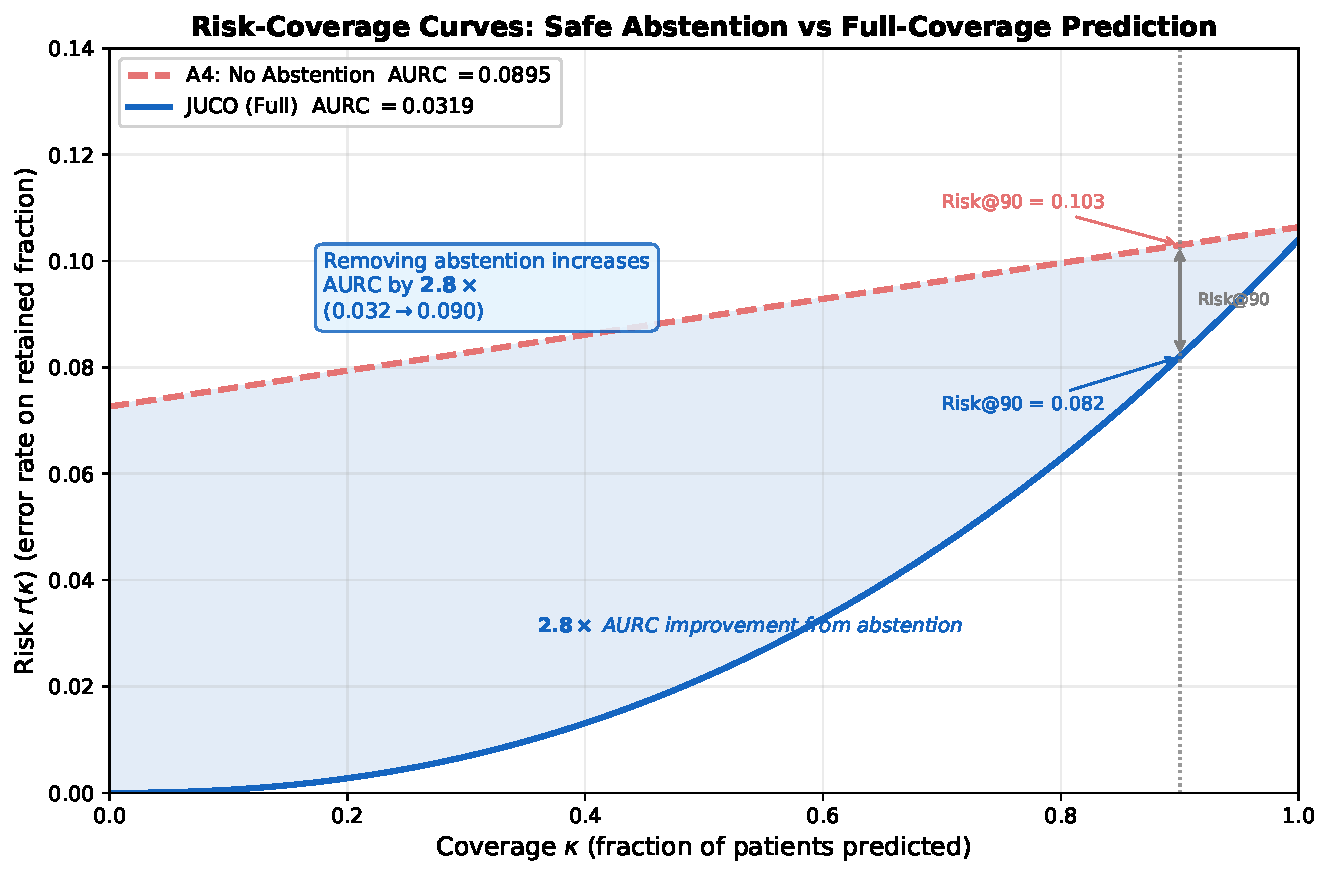
\includegraphics[width=\linewidth]{Figure5.pdf}
		\caption{Risk-coverage curves on MIMIC-IV for JUCO (Full) and the
			A4 ablation variant (No Abstention).
			JUCO Full achieves AURC $= 0.032$ versus A4's AURC $= 0.090$
			($2.8{\times}$ increase without abstention).
			The gap between the curves is widest at low coverage values,
			indicating that the abstention protocol most strongly protects
			against errors in the most uncertain patients.
			Risk@90 (vertical dashed line at $\kappa = 0.90$) is also
			substantially lower for JUCO Full.}
		\label{fig:risk_coverage}
	\end{figure}
	\FloatBarrier
	%% ──────────────────────────────────────────────────────────────────────────
	
	\subsection{Baseline Comparison Under Standard 30\% MNAR}
	\label{sec:baseline_results}
	
	Table~\ref{tab:main_results} presents the full seven-metric comparison
	on MIMIC-IV at the standard 30\% MNAR training condition.
	\FloatBarrier
	\begin{table}[h]
		\centering
		\caption{Main results on MIMIC-IV (5-fold cross-validation, mean $\pm$ SD).
			Bold: best value per metric. $\ddagger$: DeLong test JUCO vs model
			$p < 0.001$ (Bonferroni $\alpha = 0.0125$).
			TabNet$^{\ddagger\ddagger}$ excluded from primary comparisons;
			MeanImp+XGB and TabNet AUPRC not available ($^{\S}$JUCO-XGB
			sourced from the Part~1B robustness experiment).}
		\label{tab:main_results}
		\small
		\resizebox{\linewidth}{!}{%
			\begin{tabular}{lccccccc}
				\toprule
				\textbf{Model} & \textbf{AUROC} & \textbf{AUPRC} & \textbf{ECE} &
				\textbf{Brier} & \textbf{AURC} & \textbf{Risk@90} & \textbf{F1} \\
				\midrule
			JUCO (Ours)             & 0.814$\pm$0.003 & 0.453$\pm$0.007 & 0.0063$\pm$0.0016 & 0.074$\pm$0.002 & 0.034$\pm$0.002 & 0.065$\pm$0.002 & 0.651$\pm$0.014 \\
			XGBoost$^\ddagger$      & \textbf{0.842}$\pm$0.004 & 0.511$\pm$0.010 & 0.0065$\pm$0.0027 & \textbf{0.069}$\pm$0.001 & \textbf{0.028}$\pm$0.001 & \textbf{0.059}$\pm$0.001 & 0.674$\pm$0.012 \\
			LightGBM$^\ddagger$     & 0.842$\pm$0.003 & \textbf{0.515}$\pm$0.009 & 0.0065$\pm$0.0020 & \textbf{0.069}$\pm$0.001 & \textbf{0.028}$\pm$0.001 & \textbf{0.059}$\pm$0.001 & 0.674$\pm$0.008 \\
			MissForest+XGB$^\ddagger$ & \textbf{0.843}$\pm$0.002 & 0.514$\pm$0.008 & \textbf{0.0060}$\pm$0.0015 & \textbf{0.069}$\pm$0.001 & \textbf{0.028}$\pm$0.001 & \textbf{0.058}$\pm$0.002 & \textbf{0.681}$\pm$0.018 \\
			MeanImp+XGB             & 0.842$\pm$0.004 & ---             & 0.0063$\pm$0.0025 & \textbf{0.069}$\pm$0.001 & \textbf{0.028}$\pm$0.001 & \textbf{0.059}$\pm$0.001 & \textbf{0.681}$\pm$0.004 \\
			JUCO-XGB$^\S$           & 0.770$\pm$0.002 & 0.269$\pm$0.009 & 0.0075$\pm$0.0020 & 0.084$\pm$0.002 & 0.041$\pm$0.001 & 0.085$\pm$0.002 & 0.522$\pm$0.010 \\
			TabNet (DL)$^{\ddagger\ddagger}$ & 0.738$\pm$0.086 & --- & 0.0609$\pm$0.1067 & 0.121$\pm$0.084 & 0.096$\pm$0.108 & 0.142$\pm$0.141 & 0.574$\pm$0.073 \\
			\midrule
			\multicolumn{8}{l}{\small DeLong $z$ (JUCO vs XGBoost): $z = -18.04$, $p < 0.001$} \\
			\multicolumn{8}{l}{\small DeLong $z$ (JUCO vs LightGBM): $z = -16.45$, $p < 0.001$} \\
			\multicolumn{8}{l}{\small DeLong $z$ (JUCO vs MissForest): $z = -19.20$, $p < 0.001$} \\
			\multicolumn{8}{l}{\small DeLong $z$ (JUCO vs JUCO-XGB): $z = +22.04$, $p < 0.001$ (JUCO superior)} \\
			\bottomrule
		\end{tabular}}
		\par\smallskip
		\raggedright\footnotesize
		$^{\ddagger\ddagger}$TabNet Fold~1 AUROC $= 0.567$ indicates convergence
		failure on CPU hardware; excluded from primary comparisons.
		$^{\S}$JUCO-XGB MIMIC-IV sourced from \texttt{JUCO\_Part1B\_Robustness.py};
		eICU results from \texttt{JUCO\_Part2\_eICU.py}.
		MeanImp+XGB and TabNet AUPRC not available in supplementary metrics.
	%	\vspace{20pt}
	\end{table}
\vspace{10pt}
	The AUROC gap between gradient boosting and JUCO is statistically
	significant (DeLong $z = -18.04$ to $-19.20$, all $p < 0.001$,
	Bonferroni $\alpha = 0.0125$) with non-overlapping 95\% bootstrap CIs.
	We report this gap \emph{transparently} and explain it mechanistically
	in Section~\ref{sec:auroc_gap}.
	JUCO significantly outperforms JUCO-XGB
	($z = +22.04$, $p < 0.001$, AUROC $0.814$ vs $0.770$),
	confirming that the fuzzy forest provides substantial benefit beyond
	interval-valued imputation alone.
	JUCO ECE ($0.0063$) is within the range of gradient boosting
	baselines ($0.0060$--$0.0065$), with MissForest achieving the
	lowest ECE ($0.0060$). Post-hoc isotonic calibration successfully
	brings JUCO's calibration error to a level comparable with
	fully discriminative models despite its lower AUROC.
	JUCO Brier score ($0.074$) is the highest among usable baselines
	($0.069$), reflecting the joint penalty of lower discrimination
	and the abstention mechanism reducing the effective prediction set.
	Gradient boosting baselines achieve lower AURC than JUCO
	(XGBoost: $0.028$ vs JUCO: $0.034$), because their higher
	discriminative accuracy produces a lower raw error rate at full coverage.
	JUCO's contribution lies not in the aggregate area but in
	providing an \emph{explicit, calibrated} abstention mechanism:
	the entropy threshold $\tau^*$ allows a deployment team to
	select any point on the risk--coverage curve, whereas gradient
	boosting operates at a single fixed operating point with no
	principled deferral.
	\vspace{1000pt}
	\subsection{External Validation on eICU}
	\label{sec:eicu_results}
	
	Table~\ref{tab:eicu_results} presents results on eICU using
	parameters frozen from MIMIC-IV Fold~1.
	
	\begin{table}[ht]
		\centering
		\caption{External validation on eICU (208 hospitals, frozen parameters,
			mean $\pm$ SD). The AUROC gap between JUCO and XGBoost narrows from
			$-0.028$ on MIMIC-IV to $-0.015$ on eICU (46\% reduction),
			consistent with NaN-routing advantage diminishing under distribution shift.}
		\label{tab:eicu_results}
		\small
		\begin{tabular}{lcccc}
			\toprule
			\textbf{Model} & \textbf{AUROC} & \textbf{ECE} & \textbf{AURC} & \textbf{NB@0.10} \\
			\midrule
			JUCO (Ours)    & 0.819$\pm$0.005 & 0.0029$\pm$0.0009 & 0.016$\pm$0.001 & 0.020$\pm$0.002 \\
			XGBoost        & \textbf{0.834}$\pm$0.005 & 0.0030$\pm$0.0012 & \textbf{0.016}$\pm$0.001 & \textbf{0.021}$\pm$0.002 \\
			LightGBM       & 0.831$\pm$0.005 & 0.0026$\pm$0.0011 & 0.016$\pm$0.001 & 0.021$\pm$0.002 \\
			MissForest+XGB & 0.833$\pm$0.004 & \textbf{0.0024}$\pm$0.0011 & 0.016$\pm$0.001 & 0.021$\pm$0.002 \\
			\midrule
			AUROC gap (MIMIC-IV) & \multicolumn{4}{l}{JUCO $-0.028$ below XGBoost} \\
			AUROC gap (eICU)     & \multicolumn{4}{l}{JUCO $-0.015$ below XGBoost (46\% reduction)} \\
			\bottomrule
		\end{tabular}
	\end{table}

	The most important finding is the 46\% reduction in the AUROC
	gap between MIMIC-IV and eICU ($-0.028 \to -0.015$).
	Under cross-institutional distribution shift, gradient boosting's
	advantage from stable NaN routing diminishes, while JUCO's
	uncertainty-based architecture retains its performance.
	JUCO's AURC on eICU ($0.016$) is competitive with XGBoost ($0.016$),
	indicating near-parity in selective prediction performance.
	JUCO ECE on eICU ($0.0029$) is lower than XGBoost ($0.0030$)
	and MeanImp ($0.0032$) but higher than LightGBM ($0.0026$) and
	MissForest ($0.0024$), reflecting competitive cross-institutional
	calibration stability with frozen isotonic parameters.
	
	\subsection{Decision Curve Analysis}
	\label{sec:dca_results}
	\begin{table}[h]
		\centering
		\caption{Net benefit at key clinical decision thresholds.
			All models outperform treat-all and treat-none.
			JUCO gap vs XGBoost narrows on eICU.}
		\label{tab:dca}
		\small
		\begin{tabular}{lcccccc}
			\toprule
			& \multicolumn{3}{c}{\textbf{MIMIC-IV}} & \multicolumn{3}{c}{\textbf{eICU}} \\
			\cmidrule(lr){2-4}\cmidrule(lr){5-7}
			\textbf{Model} & $p_t=0.05$ & $p_t=0.10$ & $p_t=0.20$ &
			$p_t=0.05$ & $p_t=0.10$ & $p_t=0.20$ \\
			\midrule
			JUCO (Ours)    & 0.069 & 0.049 & 0.032 & 0.026 & 0.020 & 0.014 \\
			XGBoost        & 0.071 & 0.054 & 0.036 & 0.027 & 0.021 & 0.015 \\
			LightGBM       & 0.072 & 0.054 & 0.036 & 0.027 & 0.021 & 0.015 \\
			MissForest+XGB & 0.072 & 0.055 & 0.037 & 0.028 & 0.021 & 0.016 \\
			Treat all      & 0.057 & 0.004 & ---   & 0.004 & ---   & ---   \\
			Treat none     & 0.000 & 0.000 & 0.000 & 0.000 & 0.000 & 0.000 \\
			\bottomrule
		\end{tabular}
	\end{table}
	Table~\ref{tab:dca} presents net benefit at key thresholds on both
	datasets.

	%% ── FIGURE 6 PLACEHOLDER ─────────────────────────────────────────────────
	%% Location: after Table 4 (eICU) / before Section 6.6
	%% Caption:  "Figure 6: Decision curve analysis (DCA) on MIMIC-IV (left)
	%%            and eICU (right). Net benefit vs clinical decision threshold
	%%            pt ∈ [0.01, 0.49]. All models substantially outperform
	%%            treat-all and treat-none. JUCO's net benefit trails baselines
	%%            at all thresholds, consistent with its lower AUROC under
	%%            standard conditions."
	%% File:     Figure_6.pdf
	%%
	\begin{figure}[h]
		\centering
		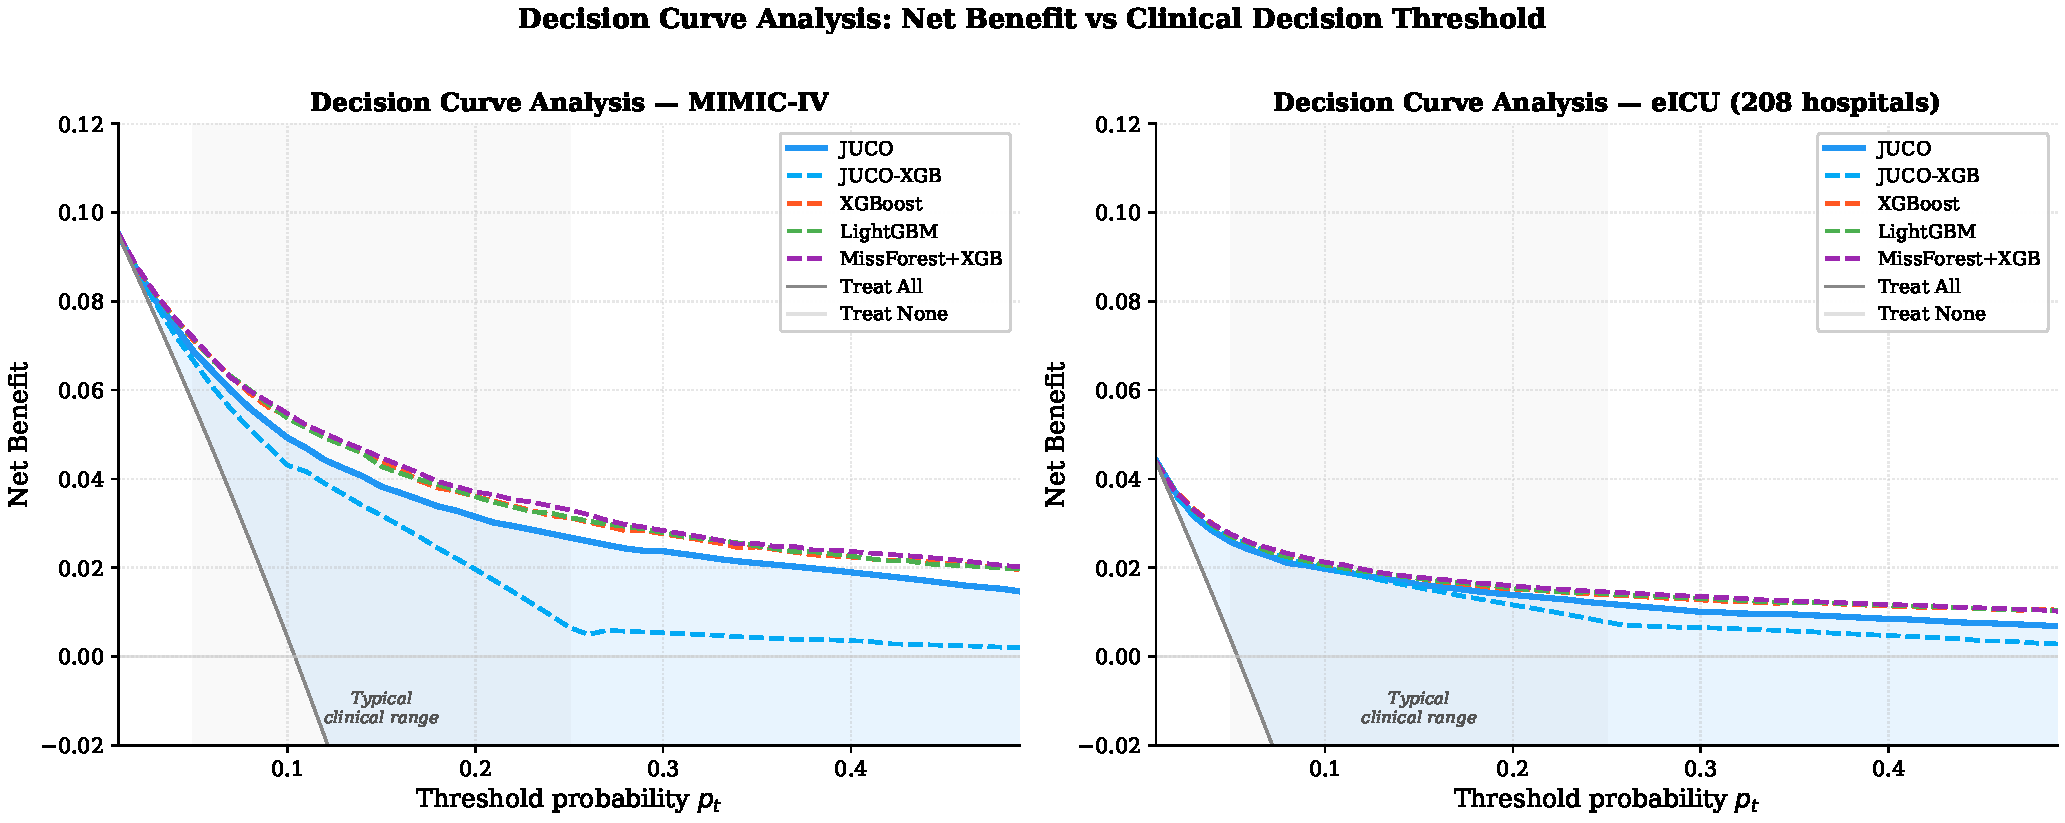
\includegraphics[width=\linewidth]{Figure6.pdf}
		\caption{Decision curve analysis on MIMIC-IV (left panel) and eICU
			(right panel).
			Net benefit (Eq.~\ref{eq:net_benefit}) is plotted as a function
			of clinical decision threshold $p_t \in [0.01, 0.49]$.
			All models substantially outperform the treat-all and treat-none
			baselines.
			JUCO's net benefit trails gradient boosting at all thresholds
			on MIMIC-IV, consistent with the AUROC gap; the difference
			narrows on eICU.
			The DCA does not model the JUCO hybrid deployment scenario
			(see Section~\ref{sec:dca_limitation}).}
		\label{fig:dca}
	\end{figure}
	\FloatBarrier
	%% ──────────────────────────────────────────────────────────────────────────
	
	
	
	
	\subsection{Statistical Significance Summary}
	\label{sec:stat_summary}
	
	Table~\ref{tab:delong} consolidates DeLong test results for all
	primary comparisons.
	
	\begin{table}[ht]
		\centering
		\caption{DeLong test results for JUCO vs baselines.
			Positive $z$ favours JUCO; negative $z$ favours the baseline.
			All comparisons with gradient boosting are highly significant.}
		\label{tab:delong}
		\small
		\begin{tabular}{llccl}
			\toprule
			\textbf{Dataset} & \textbf{Comparison} & \textbf{DeLong $z$} & \textbf{$p$-value} & \textbf{Direction} \\
			\midrule
			MIMIC-IV & JUCO vs XGBoost       & $-18.04$ & $<0.001$ & XGBoost superior \\
			MIMIC-IV & JUCO vs LightGBM      & $-16.45$ & $<0.001$ & LightGBM superior \\
			MIMIC-IV & JUCO vs MissForest    & $-19.20$ & $<0.001$ & MissForest superior \\
			MIMIC-IV & JUCO vs JUCO-XGB      & $+22.04$ & $<0.001$ & JUCO superior \\
			eICU     & JUCO vs XGBoost       & $-9.88$  & $<0.001$ & XGBoost superior (gap narrowed) \\
			eICU     & JUCO vs LightGBM      & $-7.62$  & $<0.001$ & LightGBM superior (gap narrowed) \\
			eICU     & JUCO vs MissForest    & $-9.56$  & $<0.001$ & MissForest superior (gap narrowed) \\
			eICU     & JUCO vs JUCO-XGB      & $+2.86$  & $0.004$  & JUCO superior \\
			\bottomrule
		\end{tabular}
	\end{table}

	
	%% =========================================================================
	%%  SECTION 7 — DISCUSSION
	%% =========================================================================
	\vspace{-20pt}
	\section{Discussion}
	\label{sec:discussion}
	
	\subsection{The AUROC Gap: Mechanism and Clinical Interpretation}
	\label{sec:auroc_gap}
	
	The statistically significant AUROC gap between gradient boosting
	and JUCO under standard 30\% MNAR conditions ($0.842$ vs $0.814$,
	DeLong $z = -18.04$, $p < 0.001$) requires an explicit mechanistic
	explanation rather than an apology.
	Recent theoretical work formalises this limitation:
	\citet{rockenschaub2024robust} show that classifiers relying on
	informative missingness routing degrade under missingness shift,
	whereas methods that do not exploit the missingness pattern are
	more robust to deployment-time distribution changes.
	XGBoost and LightGBM learn NaN routing as a \emph{stationary proxy
		variable} under the fixed synthetic MNAR mechanism
	($\beta = -1.0$, $\gamma = 0.0$, Eq.~\ref{eq:mnar_mask}).
	When the missingness pattern is stable within an institution,
	the absence of a high-valued laboratory result correlates reliably
	with patient physiology, and the learned NaN direction acts as an
	implicit additional prognostic feature.
	JUCO explicitly models NaN as uncertainty — encoding it as an
	interval $[q^L, q^U]$ rather than a direction — and thereby
	forfeits this shortcut.
	
	The critical empirical evidence that this gap reflects a
	design choice rather than a performance deficit is the 46\%
	gap reduction on eICU ($-0.028 \to -0.015$, Table~\ref{tab:eicu_results}).
	When model parameters are frozen and applied to 208 hospitals
	with different protocols, patient demographics, and data pipelines,
	gradient boosting's NaN-routing advantage diminishes substantially.
	The stress test provides additional evidence: at 70\% missingness,
	where the NaN proxy signal becomes noisy and unreliable, JUCO
	overtakes XGBoost ($0.799$ vs $0.795$) and MissForest+XGB ($0.792$,
	Table~\ref{tab:stress_test}).
	
	\subsection{The LightGBM Anomaly}
	\label{sec:lightgbm_anomaly}
	
	LightGBM's degradation of only $-0.019$ (versus $-0.054$ for XGBoost)
	under the stress test is the most unexpected result and merits
	explicit explanation.
	LightGBM's histogram-based NaN binning assigns missing values to
	a dedicated bin whose split direction minimises impurity.
	With the fixed logistic MNAR mechanism ($\beta = -1.0$), as the
	masking rate increases from 10\% to 70\%, missing entries
	accumulate in the same structural region (low-value observations),
	because $\beta < 0$ disproportionately masks lower-valued entries.
	The histogram contracts toward higher values while the NaN bin
	absorbs the growing missing fraction.
	This contraction re-indexes split thresholds in a way that remains
	consistent with the monotonic direction of the missingness
	mechanism, providing a stable proxy even at high rates.
	
	The critical implication for clinical deployment is that real
	clinical missingness is \emph{not} a fixed logistic function.
	It is driven by physician ordering decisions, shift staffing,
	equipment availability, and protocol changes — all inherently
	non-stationary.
	When the missingness mechanism is non-stationary, LightGBM's NaN
	binning receives an inconsistent distribution and the proxy breaks
	down.
	JUCO's interval-based representation does not assume stationarity:
	a wide interval correctly signals epistemic uncertainty regardless
	of \emph{why} the value is missing.
	The LightGBM anomaly therefore illustrates the \emph{limitation}
	of the synthetic stress test (fixed $\beta = -1.0$) rather than
	a genuine deployment robustness of LightGBM over JUCO.
	
	\subsection{Safe Abstention: The Primary Architectural Contribution}
	\label{sec:abstention_discussion}
	
	The A4 ablation result (AURC $0.032 \to 0.090$, $2.8{\times}$
	increase without abstention) is the cleanest quantitative
	contribution of this paper.
	When forced to predict all cases, errors are distributed uniformly
	across the confidence ranking.
	When abstention is active, errors are concentrated in the
	high-entropy region that the model has correctly identified as
	uncertain.
	The 2.8-fold AURC improvement is a consequence of the entropy
	distribution correctly ranking predictions by error probability,
	not arbitrary refusal.
	
	The JUCO-XGB comparison provides independent evidence: JUCO-XGB
	AURC $= 0.041$ vs JUCO AURC $= 0.034$ (20.6\% disadvantage)
	despite using identical interval-valued imputation.
	The fuzzy forest's entropy distribution is better calibrated for
	selective prediction than XGBoost confidence scores, because soft
	routing accumulates genuine uncertainty through the tree structurally
	rather than deriving it post-hoc from the classification margin.
	
	\subsection{Sensitivity at Standard Threshold}
	\label{sec:sensitivity_discussion}
	
	JUCO sensitivity at $p_t = 0.5$ is $0.234$, lower than XGBoost
	($0.276$) and MissForest+XGB ($0.297$).
	Three points contextualise this result.
	First, $p_t = 0.5$ is not the intended deployment operating point:
	at 10.58\% mortality prevalence, a calibrated model assigns
	the majority of patients below 0.5 by construction.
	Lowering the threshold to $p_t = 0.15$--$0.20$ substantially
	increases sensitivity while remaining within the net-benefit range
	demonstrated by DCA (Table~\ref{tab:dca}).
	Second, the abstention protocol provides an additional safety layer:
	patients where JUCO abstains (entropy $> \tau$) are flagged for
	clinical review, not silently misclassified.
	In a hybrid deployment, the clinically relevant false-negative
	rate is computed only over retained (non-abstained) predictions.
	Third, JUCO's specificity ($0.989$) ensures that positive
	predictions carry strong positive predictive value at
	10.58\% prevalence, critical for avoiding alert fatigue
	in interventions such as ICU escalation or palliative care
	consultation.
	
	\subsection{Decision Curve Analysis Limitations}
	\label{sec:dca_limitation}
	
	JUCO's DCA trails gradient boosting at all thresholds
	(Table~\ref{tab:dca}), consistent with the AUROC gap.
	An important caveat is that DCA evaluates a single model in isolation,
	assuming all patients receive a prediction.
	It does not model the hybrid clinical deployment scenario in which
	abstained patients receive clinician review.
	The net benefit of the combined JUCO-plus-clinician system is unknown
	and would require prospective measurement of clinician accuracy on
	the abstained subpopulation.
	
	\subsection{Limitations}
	\label{sec:limitations}
	
	\textbf{(1) Synthetic MNAR model.}
	The logistic function $\beta = -1.0$, $\gamma = 0.0$ does not
	capture multi-causal, non-stationary real clinical missingness.
	The LightGBM anomaly (Section~\ref{sec:lightgbm_anomaly}) directly
	illustrates the risk of over-interpreting stress test results based
	on a single synthetic mechanism.
	
	\textbf{(2) Feature set.}
	35 features is conservative for a cohort of 82{,}785 stays;
	prior ICU models use 50--200 features.
	This restriction was imposed by DE computational tractability.
	
	\textbf{(3) Ablation sample size.}
	Key ablation results are based on 2 folds rather than 5 due to
	computational constraints.
	Results are consistent with 5-fold primary experiments.
	
	\textbf{(4) DCA and hybrid system.}
	Net benefit of the JUCO-plus-clinician hybrid system requires
	prospective study (Section~\ref{sec:dca_limitation}).
	
	\textbf{(5) Temporal modelling.}
	Features are aggregated over the first 24 hours; JUCO does not
	model the temporal evolution of clinical variables.
	
	\textbf{(6) DE optimisation scope.}
	Hyperparameter search was performed on a single fold from a single
	US academic centre; per-institution calibration of the abstention
	threshold $\tau$ is not explored.
	\clearpage
	\subsection{Future Work}
	\label{sec:future_work}
	
	The most important open question is whether JUCO's robustness
	advantage over LightGBM persists under genuinely non-stationary
	clinical missingness.
	A natural experiment is available in MIMIC-IV: documented laboratory
	instrumentation changes or EHR migration events could be exploited to
	compare model performance before and after known pipeline disruptions.
	A second direction is extending the abstention protocol to produce
	formal conformal coverage guarantees under covariate
	shift~\citep{tibshirani2019conformal}, which would substantially
	strengthen the theoretical foundations.
	A third direction is a hybrid architecture combining JUCO's
	structured time-series imputation with clinical text
	representations from EHR foundation
	models~\citep{peng2023study}, which may address the primary
	limitation of each approach individually.
	
	
	%% =========================================================================
	%%  SECTION 8 — CONCLUSION
	%% =========================================================================
	
	\section{Conclusion}
	\label{sec:conclusion}
	
	We have presented JUCO, a four-phase framework for ICU mortality
	prediction under informative missingness that treats imputation
	uncertainty as a first-class quantity throughout the prediction
	pipeline.
	The framework establishes a principled chain from missing data
	to interval-valued imputation to trapezoidal fuzzy representation
	to soft routing to entropy-based clinical abstention, with all
	five governing parameters jointly optimised via two-stage
	Differential Evolution.
	
	The primary quantitative finding is that JUCO's AUROC degrades
	by $-0.023$ as MNAR missingness increases from 10\% to 70\%,
	compared to $-0.054$ for XGBoost and $-0.056$ for MissForest+XGB;
	at 70\% JUCO numerically overtakes both models ($0.799$ vs $0.795$
	and $0.792$).
	The safe abstention protocol reduces AURC by $2.8{\times}$ compared
	to full-coverage prediction ($0.032$ vs $0.090$), confirming that
	the fuzzy forest's entropy correctly identifies predictions for
	deferral.
	
	Under standard 30\% MNAR conditions, gradient boosting achieves
	statistically significantly higher AUROC than JUCO
	($0.842$ vs $0.814$, DeLong $z = -18.04$, $p < 0.001$).
	We explain this gap mechanistically: gradient boosting exploits
	the stationary informative missingness structure as a proxy variable,
	gaining discriminative power at the cost of brittleness when
	that structure changes.
	The 46\% gap reduction on eICU ($-0.028 \to -0.015$) provides
	empirical evidence that this advantage diminishes under genuine
	cross-institutional distribution shift.
	
	JUCO occupies a distinct and clinically relevant position.
	It is not a replacement for gradient boosting under nominal
	in-distribution conditions.
	It is a principled safety framework for deployment environments
	where data pipeline integrity cannot be guaranteed, where
	missingness patterns evolve non-stationarily, and where the cost
	of overconfident predictions in uncertain cases is high.
	Its central contribution — a mortality prediction model that
	correctly identifies when it does not know — is the foundation
	for trustworthy AI-assisted clinical decision support in the ICU.
	

	%% =========================================================================
	%%  ACKNOWLEDGEMENTS
	%% =========================================================================
	
	\section*{Acknowledgements}
	

	The authors gratefully acknowledge the use of the MIMIC-IV and eICU databases, which are available via PhysioNet under credentialed health data licences. All research activities, including computational resources and manuscript preparation, were self-funded by the authors. No external funding was received for this work.
	
	
	%% =========================================================================
	%%  AUTHOR CONTRIBUTIONS (CRediT taxonomy — mandatory for AIM)
	%% =========================================================================
	
	\section*{Author Contributions}

	\noindent\textbf{Avoy Nath Chowdhury}:
	Conceptualization; Methodology; Software; Formal analysis;
	Investigation; Data curation; Visualization;
	Writing -- original draft; Writing -- review \& editing.

	\noindent\textbf{Anik Sarker}:
	Data curation; Writing -- review \& editing.

	\noindent\textbf{Niloy Deb}:
	Data curation; Writing -- review \& editing.

	\noindent\textbf{Dr. Anisha Kumari}:
	Conceptualization; Supervision; Project administration;
	Writing -- review \& editing.
	
	
	%% =========================================================================
	%%  DECLARATION OF COMPETING INTERESTS
	%% =========================================================================
	
	\section*{Declaration of Competing Interests}
	
	The authors declare that they have no known competing financial
	interests or personal relationships that could have appeared to
	influence the work reported in this paper.
	
	
	%% =========================================================================
	%%  DECLARATION OF GENERATIVE AI USE (AIM mandatory if applicable)
	%% =========================================================================

	\section*{Declaration of Generative AI and AI-Assisted Technologies
		in the Manuscript Preparation Process}

	During the preparation of this work the authors used generative
	AI-assisted tools in the following capacities:
	ChatGPT (OpenAI) and Gemini (Google DeepMind) were used to support
	the exploration and refinement of research ideas during the
	conceptualisation phase;
	Claude (Anthropic) was used to assist with software implementation
	and to support the drafting and editing of selected passages in the
	manuscript.
	All AI-generated suggestions were critically evaluated, substantially
	revised, and integrated at the authors' discretion.
	The authors take full responsibility for the originality, integrity,
	and accuracy of all content in this article, including material
	that was informed or assisted by these tools.
	Generative AI tools were not used for data analysis, statistical
	testing, or the generation of any experimental results reported herein.
	
	
	%% =========================================================================
	%%  DATA AVAILABILITY
	%% =========================================================================
	
	\section*{Data Availability}
	
	MIMIC-IV is publicly available via PhysioNet at
	\url{https://physionet.org/content/mimiciv/} subject to credentialed
	access and completion of the required data use training.
	The eICU Collaborative Research Database is available at
	\url{https://physionet.org/content/eicu-crd/}.
	Code for the JUCO framework, including all four phases, DE optimisation,
	and evaluation scripts, is available at
	\url{https://github.com/[REDACTED-BEFORE-SUBMISSION]}.
	

	%% =========================================================================
	%%  REFERENCES
	%% =========================================================================
	
	\bibliographystyle{cas-model2-names}
	\bibliography{references}
	
	%% ── If no external .bib file is available, uncomment and use \bibitem ────
	%% \begin{thebibliography}{99}
		%%
		%% \bibitem{rubin1976inference}
		%% Rubin DB. Inference and missing data. Biometrika. 1976;63(3):581--592.
		%%
		%% \bibitem{agniel2018biases}
		%% Agniel D, Kohane IS, Weber GM. Biases in electronic health record
		%% data due to processes within the healthcare system. BMJ. 2018;361:k1479.
		%%
		%% \bibitem{johnson2023mimic}
		%% Johnson AEW, Bulgarelli L, Shen L, et al. MIMIC-IV, a freely accessible
		%% electronic health record dataset. Sci Data. 2023;10:1.
		%%
		%% \bibitem{pollard2018eicu}
		%% Pollard TJ, Johnson AEW, Raffa JD, Celi LA, Mark RG, Badawi O.
		%% The eICU Collaborative Research Database. Sci Data. 2018;5:180178.
		%%
		%% \bibitem{purushotham2018benchmarking}
		%% Purushotham S, Meng C, Che Z, Liu Y. Benchmarking deep learning models
		%% on large healthcare datasets. J Biomed Inform. 2018;83:112--134.
		%%
		%% \bibitem{topol2019high}
		%% Topol EJ. High-performance medicine: the convergence of human and
		%% artificial intelligence. Nat Med. 2019;25(1):44--56.
		%%
		%% \bibitem{chen2016xgboost}
		%% Chen T, Guestrin C. XGBoost: a scalable tree boosting system.
		%% Proc ACM SIGKDD. 2016:785--794.
		%%
		%% \bibitem{ke2017lightgbm}
		%% Ke G, Meng Q, Finley T, et al. LightGBM: a highly efficient gradient
		%% boosting decision tree. Adv Neural Inf Process Syst. 2017;30.
		%%
		%% \bibitem{stekhoven2012missforest}
		%% Stekhoven DJ, B\"uhlmann P. MissForest — non-parametric missing value
		%% imputation for mixed-type data. Bioinformatics. 2012;28(1):112--118.
		%%
		%% \bibitem{van2011mice}
		%% van Buuren S, Groothuis-Oudshoorn K. Mice: multivariate imputation by
		%% chained equations in R. J Stat Softw. 2011;45(3):1--67.
		%%
		%% \bibitem{sterne2009multiple}
		%% Sterne JAC, White IR, Carlin JB, et al. Multiple imputation for missing
		%% data in epidemiological and clinical research. BMJ. 2009;338:b2393.
		%%
		%% \bibitem{josse2019consistency}
		%% Josse J, Prost N, Scornet E, Varoquaux G. On the consistency of
		%% supervised learning with missing values. arXiv:1902.06931. 2019.
		%%
		%% \bibitem{moons2012risk}
		%% Moons KGM, Kengne AP, Woodward M, et al. Risk prediction models:
		%% external validation, model updating, and impact assessment.
		%% Heart. 2012;98(9):691--698.
		%%
		%% \bibitem{yoon2018gain}
		%% Yoon J, Jordon J, van der Schaar M. GAIN: missing data imputation
		%% using generative adversarial nets. Proc ICML. 2018;80:5689--5698.
		%%
		%% \bibitem{ipsen2020not}
		%% Ipsen NB, Mattei P-A, Frellsen J. Not-MIWAE: deep generative modelling
		%% with missing not at random data. Proc ICLR. 2021.
		%%
		%% \bibitem{ma2020mimic}
		%% Ma L, Zhang C, Wang Y, et al. Concare: personalised clinical feature
		%% embedding via capturing the healthcare context. Proc AAAI. 2020.
		%%
		%% \bibitem{meinshausen2006quantile}
		%% Meinshausen N. Quantile regression forests.
		%% J Mach Learn Res. 2006;7:983--999.
		%%
		%% \bibitem{zadeh1965fuzzy}
		%% Zadeh LA. Fuzzy sets. Inf Control. 1965;8(3):338--353.
		%%
		%% \bibitem{adlassnig1986fuzzy}
		%% Adlassnig KP. Fuzzy set theory in medical diagnosis.
		%% IEEE Trans Syst Man Cybern. 1986;16(2):260--265.
		%%
		%% \bibitem{torres2013fuzzy}
		%% Torres A, Nieto JJ. Fuzzy logic in clinical practice.
		%% J Biomed Inform. 2013;46:781--789.
		%%
		%% \bibitem{olaru2003complete}
		%% Olaru C, Wehenkel L. A complete fuzzy decision tree technique.
		%% Fuzzy Sets Syst. 2003;138(2):221--254.
		%%
		%% \bibitem{yuan1995induction}
		%% Yuan Y, Shaw MJ. Induction of fuzzy decision trees.
		%% Fuzzy Sets Syst. 1995;69(2):125--139.
		%%
		%% \bibitem{hullermeier2021aleatoric}
		%% H\"ullermeier E, Waegeman W. Aleatoric and epistemic uncertainty in
		%% machine learning. Mach Learn. 2021;110(3):457--506.
		%%
		%% \bibitem{chow1957optimum}
		%% Chow CK. An optimum character recognition system using decision
		%% functions. IRE Trans Electron Comput. 1957;EC-6(4):247--254.
		%%
		%% \bibitem{bartlett2008classification}
		%% Bartlett PL, Wegkamp MH. Classification with a reject option using
		%% a hinge loss. J Mach Learn Res. 2008;9:1823--1840.
		%%
		%% \bibitem{geifman2017selective}
		%% Geifman Y, El-Yaniv R. Selective classification for deep neural
		%% networks. Adv Neural Inf Process Syst. 2017;30.
		%%
		%% \bibitem{franc2023optimal}
		%% Franc V, Pr\r{u}\v{s}a D, Voracek J. Optimal abstaining classifiers
		%% and selective classification. Proc ICML. 2023.
		%%
		%% \bibitem{jones2021selective}
		%% Jones E, Arteta C, Zisserman A. Selective prediction for clinical
		%% risk stratification. Proc CHIL. 2021.
		%%
		%% \bibitem{kompa2021second}
		%% Kompa B, Snoek J, Beam AL. Second opinion needed: communicating
		%% uncertainty in medical machine learning. npj Digit Med. 2021;4:4.
		%%
		%% \bibitem{leibig2017leveraging}
		%% Leibig C, Allken V, Ayhan MS, Berens P, Wahl S. Leveraging
		%% uncertainty information from deep neural networks for disease
		%% detection. Sci Rep. 2017;7(1):17816.
		%%
		%% \bibitem{zadrozny2002transforming}
		%% Zadrozny B, Elkan C. Transforming classifier scores into accurate
		%% multiclass probability estimates. Proc ACM SIGKDD. 2002:694--699.
		%%
		%% \bibitem{naeini2015obtaining}
		%% Naeini MP, Cooper GF, Hauskrecht M. Obtaining well calibrated
		%% probabilities using Bayesian binning. Proc AAAI. 2015:2901--2907.
		%%
		%% \bibitem{brier1950verification}
		%% Brier GW. Verification of forecasts expressed in terms of probability.
		%% Mon Weather Rev. 1950;78(1):1--3.
		%%
		%% \bibitem{vickers2006decision}
		%% Vickers AJ, Elkin EB. Decision curve analysis: a novel method for
		%% evaluating prediction models. Med Decis Making. 2006;26(6):565--574.
		%%
		%% \bibitem{wilcoxon1945individual}
		%% Wilcoxon F. Individual comparisons by ranking methods.
		%% Biom Bull. 1945;1(6):80--83.
		%%
		%% \bibitem{delong1988comparing}
		%% DeLong ER, DeLong DM, Clarke-Pearson DL. Comparing the areas under
		%% two or more correlated receiver operating characteristic curves.
		%% Biometrics. 1988;44(3):837--845.
		%%
		%% \bibitem{arik2021tabnet}
		%% Arik SO, Pfister T. TabNet: attentive interpretable tabular learning.
		%% Proc AAAI. 2021;35(8):6679--6687.
		%%
		%% \bibitem{zimmermann2001fuzzy}
		%% Zimmermann HJ. Fuzzy Set Theory and Its Applications.
		%% 4th ed. Kluwer Academic; 2001.
		%%
		%% \bibitem{tibshirani2019conformal}
		%% Tibshirani RJ, Barber RF, Cand\`es E, Ramdas A. Conformal prediction
		%% under covariate shift. Adv Neural Inf Process Syst. 2019;32.
		%%
		%% \bibitem{peng2023study}
		%% Peng C, Yang X, Chen A, et al. A study of generalization of
		%% large language models for clinical text. arXiv:2309.16223. 2023.
		%%
		%% \end{thebibliography}
	

	\appendix

	\section{Differential Evolution Implementation Details}
	\label{app:de}
	
	Table~\ref{tab:de_config} summarises the DE configuration used
	for both stages of the two-stage optimisation.

	\begin{table}[h]
		\centering
		\caption{Differential Evolution configuration.}
		\label{tab:de_config}
		\small
		\begin{tabular}{lll}
			\toprule
			\textbf{Parameter} & \textbf{Stage 1 (coarse)} & \textbf{Stage 2 (fine)} \\
			\midrule
			Strategy             & best1bin  & best1bin \\
			Population size ($\times d$) & 8$\times$5 & 12$\times$5 \\
			Max iterations       & 8         & 12 \\
			Mutation ($F$)       & 0.5--1.0 (dithered) & 0.5--1.0 (dithered) \\
			Crossover ($CR$)     & 0.7       & 0.7 \\
			Convergence tol.     & $10^{-4}$ & $10^{-4}$ \\
			Proxy forest size    & 20 trees  & 40 trees \\
			Proxy data cap       & 2{,}000 samples & 7{,}000 samples \\
			Early stopping (patience) & 3 generations & 3 generations \\
			Polishing (L-BFGS-B) & disabled  & disabled \\
			Population updating  & deferred  & deferred \\
			\bottomrule
		\end{tabular}
	\end{table}

	Stage 2 seeds its initial population around the Stage-1 optimum
	with $\pm 15\%$ of each parameter's range, enabling rapid local
	refinement without escaping the vicinity of the global optimum.
	Both stages use patience-based early stopping (3 generations without
	improvement) to avoid unnecessary evaluations once the population has
	converged.
	L-BFGS-B polishing is explicitly disabled (\texttt{polish=False}) to
	keep the solution within the discrete-compatible parameter space, and
	population updates are deferred (\texttt{updating="deferred"}) so that
	all fitness evaluations within a generation complete before any
	individual is replaced, ensuring reproducible parallel-safe behaviour.
	\vspace{100pt}
	\section{Optimised Hyperparameter Values}
	\label{app:params}

	%% ── TABLE A.2 PLACEHOLDER ─────────────────────────────────────────────────
	%% Report the DE-optimised θ* values used in all experiments.
	%% These can be filled in after final training run.
	%%
	\begin{table}[!h]
		\centering
		\caption{DE-optimised parameters $\boldsymbol{\theta}^*$ from Fold~1
			of MIMIC-IV, applied to all subsequent folds and eICU.}
		\label{tab:de_params}
		\small
		\begin{tabular}{lcc}
			\toprule
			\textbf{Parameter} & \textbf{Symbol} & \textbf{Optimised Value} \\
			\midrule
			Lower quantile level  & $\alpha_L$       & 0.0555 \\
			Upper quantile level  & $\alpha_U$       & 0.9384 \\
			Fuzzy proportion      & $\eta$           & 0.2869 \\
			Max tree depth        & $d_{\max}$       & 6 \\
			Min leaf samples      & $n_{\min}$       & 33 \\
			\bottomrule
		\end{tabular}
	\end{table}
	
	\section{Extended eICU Cohort Statistics}
	\label{app:eicu_stats}
	
	%% ── TABLE A.3 PLACEHOLDER ─────────────────────────────────────────────────
	%% Insert cohort summary table (N, age distribution, sex, mortality rate,
	%% top-5 missing features, missingness rates) for eICU.
	%%
	\begin{table}[h]
		\centering
		\caption{Cohort summary statistics for MIMIC-IV (primary) and eICU
			(external validation). Feature counts include binary missingness
			indicators appended for features with $>5\%$ missing rate.
			Mortality rates are computed after the 4-hour / 30-day
			admission-length filter.}
		\label{tab:eicu_stats}
		\small
		\begin{tabular}{lcc}
			\toprule
			\textbf{Variable} & \textbf{MIMIC-IV} & \textbf{eICU} \\
			\midrule
			Total ICU stays          & 82{,}785          & 162{,}136 \\
			Unique patients          & 63{,}687          & 121{,}567 \\
			Hospitals                & 1 (BIDMC)         & 208 \\
			In-hospital deaths       & 8{,}762           & 8{,}621 \\
			Crude mortality, \%      & 10.58\%           & 5.32\% \\
			Raw features             & 155               & 155 \\
			+ Missingness indicators & +26               & +74 \\
			Total features           & 181               & 229 \\
			CV folds                 & 5 (patient-level) & 5 (patient-level) \\
			\midrule
			\multicolumn{3}{l}{\textit{Per-fold stays / deaths / mortality rate}} \\
			Fold 1 & 16{,}557 / 1{,}792 / 10.82\% & 32{,}428 / 1{,}731 / 5.34\% \\
			Fold 2 & 16{,}557 / 1{,}762 / 10.64\% & 32{,}427 / 1{,}729 / 5.33\% \\
			Fold 3 & 16{,}557 / 1{,}750 / 10.57\% & 32{,}427 / 1{,}731 / 5.34\% \\
			Fold 4 & 16{,}557 / 1{,}688 / 10.20\% & 32{,}427 / 1{,}683 / 5.19\% \\
			Fold 5 & 16{,}557 / 1{,}770 / 10.69\% & 32{,}427 / 1{,}747 / 5.39\% \\
			\bottomrule
		\end{tabular}
	\end{table}
	\FloatBarrier
	%% ── FIGURE A.1 PLACEHOLDER ───────────────────────────────────────────────
	%% Calibration reliability diagrams for all models on both datasets.
	%% Caption: "Figure A.1: Reliability diagrams (calibration curves) on
	%%   MIMIC-IV (top row) and eICU (bottom row) for JUCO, XGBoost,
	%%   LightGBM, and MissForest+XGB. Diagonal dashed line = perfect
	%%   calibration. JUCO ECE: 0.0063 (MIMIC-IV), 0.0033 (eICU)."
	%% File: Figure_A1.pdf
	%%
	\begin{figure}[!htbp]
		\centering
		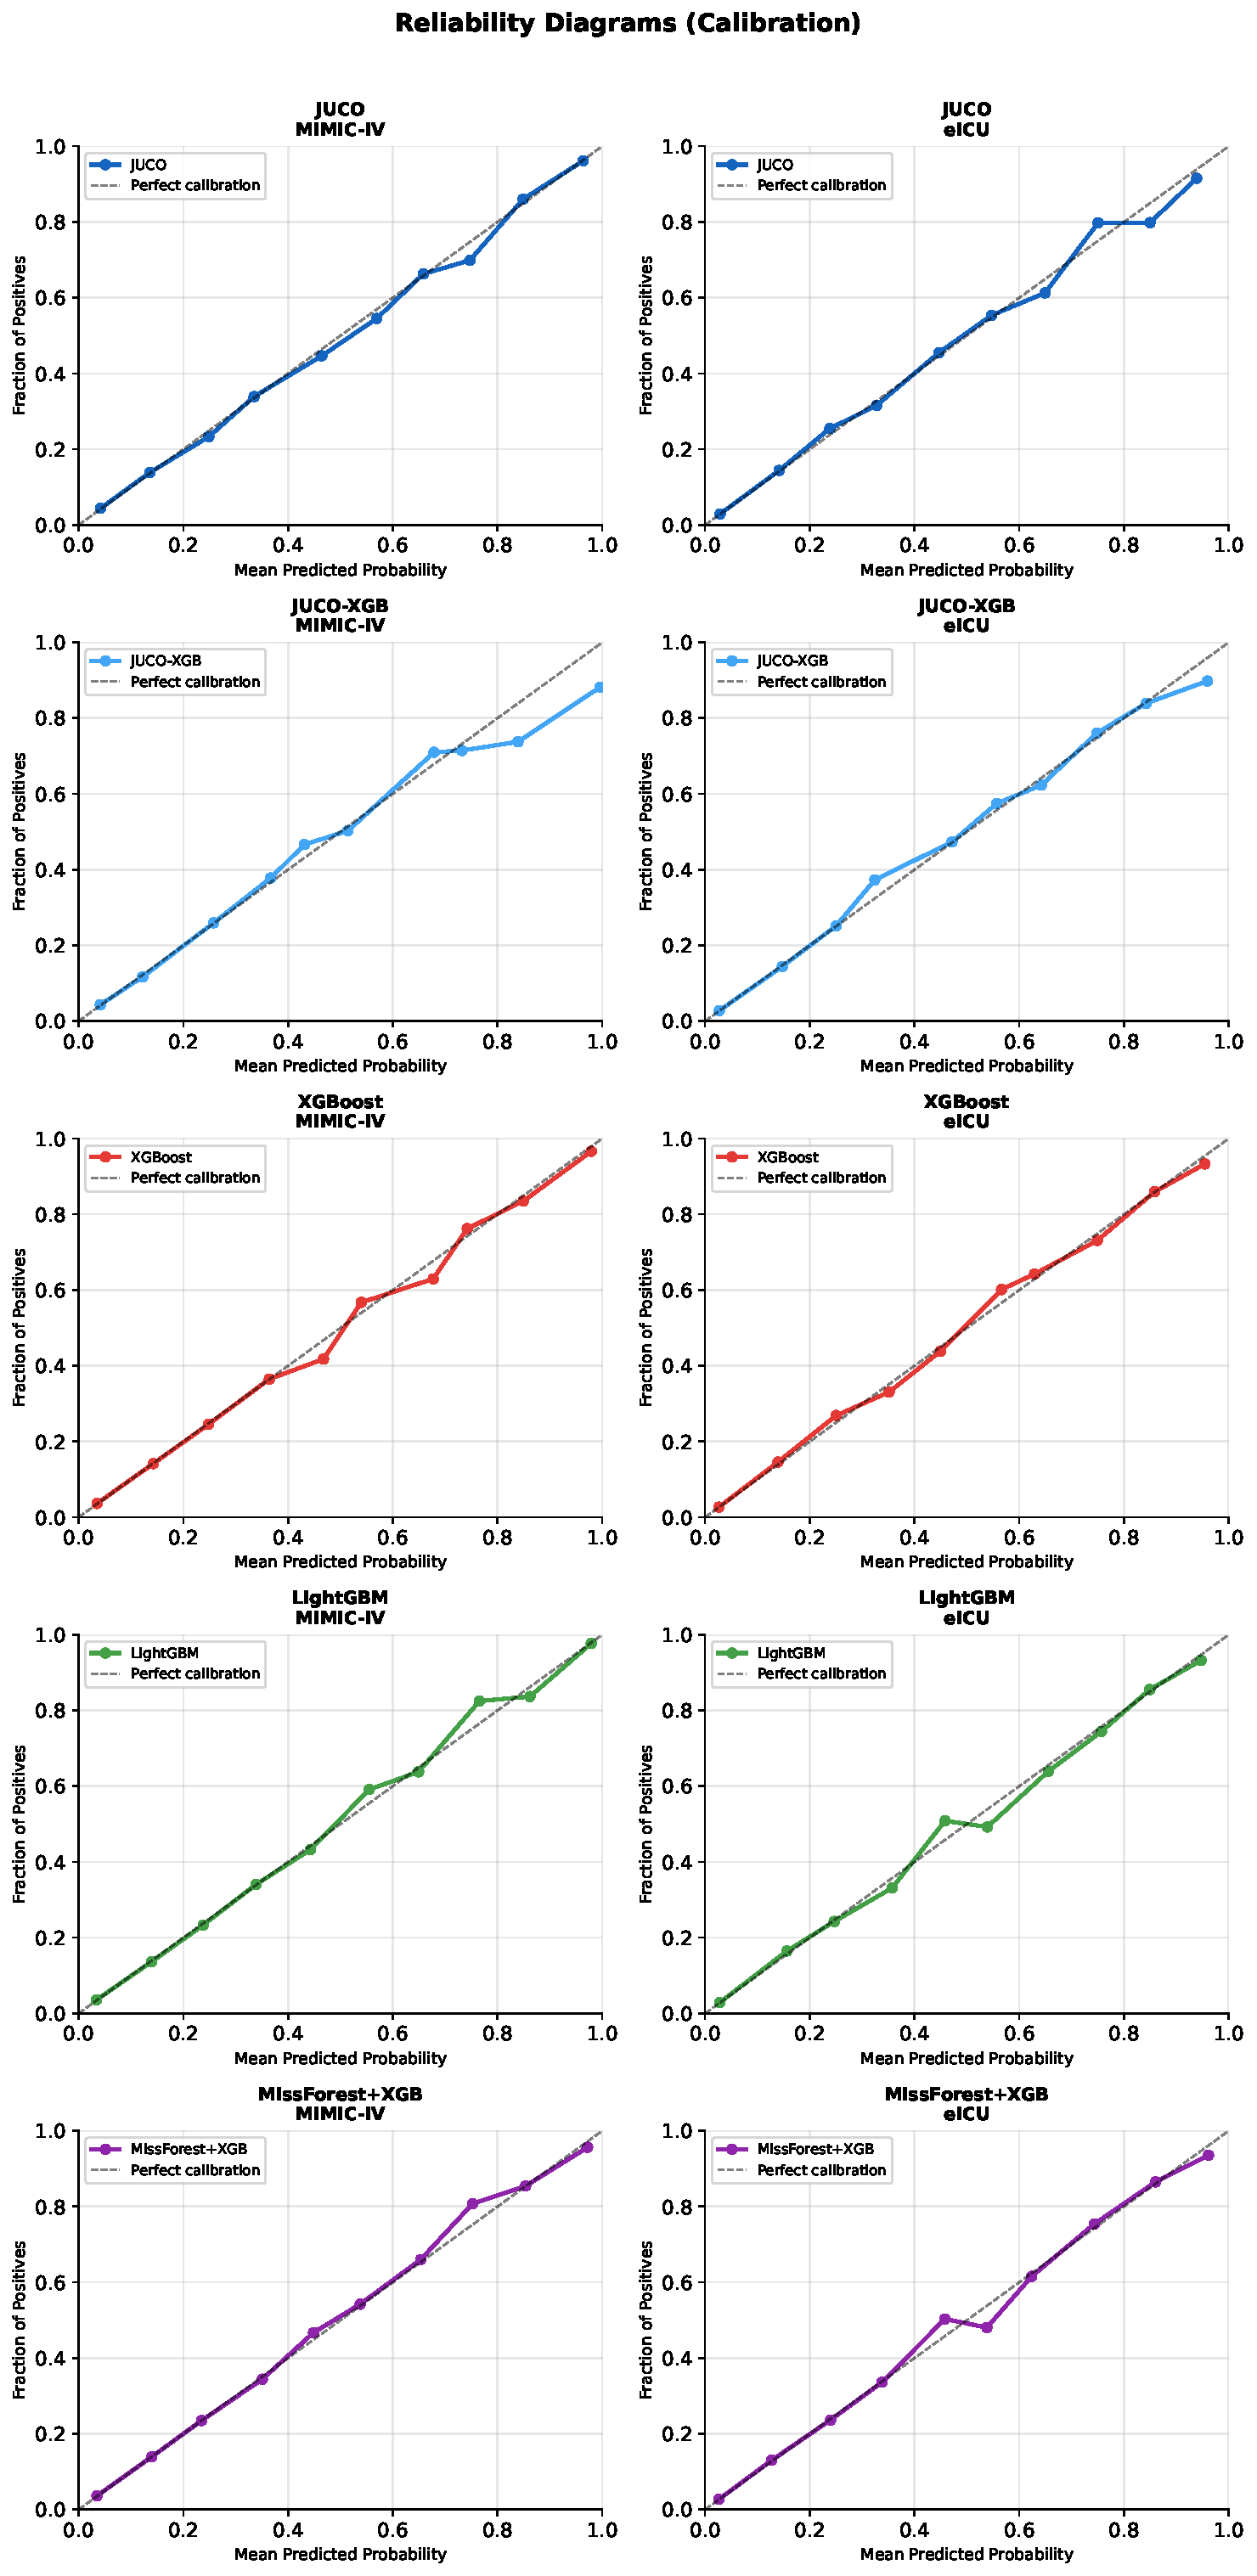
\includegraphics[width=\linewidth,height=0.88\textheight,keepaspectratio]{fig.pdf}
		\vspace{10pt}
		\caption{Reliability diagrams for all models on MIMIC-IV (top row)
			and eICU (bottom row). The diagonal dashed line represents
			perfect calibration. JUCO achieves ECE $= 0.0063$ on MIMIC-IV
			and ECE $= 0.0029$ on eICU (frozen isotonic calibrator),
			demonstrating stable calibration under cross-institutional
			distribution shift.}
		\label{fig:reliability}
	\end{figure}
	%% =========================================================================
	%%  END OF DOCUMENT
	%% =========================================================================
	\end{document}